% Options for packages loaded elsewhere
\PassOptionsToPackage{unicode}{hyperref}
\PassOptionsToPackage{hyphens}{url}
%
\documentclass[
  12pt,
]{article}
\usepackage{amsmath,amssymb}
\usepackage{lmodern}
\usepackage{iftex}
\ifPDFTeX
  \usepackage[T1]{fontenc}
  \usepackage[utf8]{inputenc}
  \usepackage{textcomp} % provide euro and other symbols
\else % if luatex or xetex
  \usepackage{unicode-math}
  \defaultfontfeatures{Scale=MatchLowercase}
  \defaultfontfeatures[\rmfamily]{Ligatures=TeX,Scale=1}
  \setmainfont[]{Times New Roman}
\fi
% Use upquote if available, for straight quotes in verbatim environments
\IfFileExists{upquote.sty}{\usepackage{upquote}}{}
\IfFileExists{microtype.sty}{% use microtype if available
  \usepackage[]{microtype}
  \UseMicrotypeSet[protrusion]{basicmath} % disable protrusion for tt fonts
}{}
\makeatletter
\@ifundefined{KOMAClassName}{% if non-KOMA class
  \IfFileExists{parskip.sty}{%
    \usepackage{parskip}
  }{% else
    \setlength{\parindent}{0pt}
    \setlength{\parskip}{6pt plus 2pt minus 1pt}}
}{% if KOMA class
  \KOMAoptions{parskip=half}}
\makeatother
\usepackage{xcolor}
\usepackage[margin=1in]{geometry}
\usepackage{graphicx}
\makeatletter
\def\maxwidth{\ifdim\Gin@nat@width>\linewidth\linewidth\else\Gin@nat@width\fi}
\def\maxheight{\ifdim\Gin@nat@height>\textheight\textheight\else\Gin@nat@height\fi}
\makeatother
% Scale images if necessary, so that they will not overflow the page
% margins by default, and it is still possible to overwrite the defaults
% using explicit options in \includegraphics[width, height, ...]{}
\setkeys{Gin}{width=\maxwidth,height=\maxheight,keepaspectratio}
% Set default figure placement to htbp
\makeatletter
\def\fps@figure{htbp}
\makeatother
\setlength{\emergencystretch}{3em} % prevent overfull lines
\providecommand{\tightlist}{%
  \setlength{\itemsep}{0pt}\setlength{\parskip}{0pt}}
\setcounter{secnumdepth}{-\maxdimen} % remove section numbering
\newlength{\cslhangindent}
\setlength{\cslhangindent}{1.5em}
\newlength{\csllabelwidth}
\setlength{\csllabelwidth}{3em}
\newlength{\cslentryspacingunit} % times entry-spacing
\setlength{\cslentryspacingunit}{\parskip}
\newenvironment{CSLReferences}[2] % #1 hanging-ident, #2 entry spacing
 {% don't indent paragraphs
  \setlength{\parindent}{0pt}
  % turn on hanging indent if param 1 is 1
  \ifodd #1
  \let\oldpar\par
  \def\par{\hangindent=\cslhangindent\oldpar}
  \fi
  % set entry spacing
  \setlength{\parskip}{#2\cslentryspacingunit}
 }%
 {}
\usepackage{calc}
\newcommand{\CSLBlock}[1]{#1\hfill\break}
\newcommand{\CSLLeftMargin}[1]{\parbox[t]{\csllabelwidth}{#1}}
\newcommand{\CSLRightInline}[1]{\parbox[t]{\linewidth - \csllabelwidth}{#1}\break}
\newcommand{\CSLIndent}[1]{\hspace{\cslhangindent}#1}
\usepackage{floatrow}
\floatsetup[figure]{capposition=top}
\usepackage{float}
\floatplacement{figure}{H}
\usepackage[T1]{fontenc}
\usepackage[utf8]{inputenc}
\providecommand{\keywords}[1]{\textbf{Keywords:} #1}
\providecommand{\wordcount}[1]{\text{Word Count:}#1} 

\usepackage{booktabs}
\usepackage{longtable}
\usepackage{array}
\usepackage{multirow}
\usepackage{wrapfig}
\usepackage{float}
\usepackage{colortbl}
\usepackage{pdflscape}
\usepackage{tabu}
\usepackage{threeparttable}
\usepackage{threeparttablex}
\usepackage[normalem]{ulem}
\usepackage{makecell}
\usepackage{xcolor}
\ifLuaTeX
  \usepackage{selnolig}  % disable illegal ligatures
\fi
\IfFileExists{bookmark.sty}{\usepackage{bookmark}}{\usepackage{hyperref}}
\IfFileExists{xurl.sty}{\usepackage{xurl}}{} % add URL line breaks if available
\urlstyle{same} % disable monospaced font for URLs
\hypersetup{
  pdftitle={How has the Brazilian Amazon been constructed as a problem:Presidential speeches and transnational politics since 1985},
  pdfauthor={Livio Silva-Muller; Henrique Sposito},
  hidelinks,
  pdfcreator={LaTeX via pandoc}}

\title{How has the Brazilian Amazon been constructed as a
problem:Presidential speeches and transnational politics since 1985}
\author{Livio Silva-Muller \and Henrique Sposito\footnote{Both
  co-authors contributed equally to the article. Names are ordered
  alphabetically. Livio is a PhD Candidate in Anthropology and Sociology
  at the Geneva Graduate Institute and affiliated to the Albert
  Hirschman Centre on Democracy. Henrique is a PhD Candidate in
  International Relations and Political Sciences at the Geneva Graduate
  Institute and affiliated to the Centre for International Environmental
  Studies.}}
\date{20 September 2022}

\begin{document}
\maketitle
\begin{abstract}
Presidential speeches influence the ways we think about and act towards
the environment transnationally, but they are understudied. We propose a
framework to investigate how the Brazilian Amazon has been constructed
as a problem in discourses across time and space. Using supervised
machine learning, we classify statements about the Amazon in 6130
presidential speeches since 1985. We find that national and
international events drive the frequency at which the topic of the
Amazon is mentioned in presidential speeches inside and outside Brazil.
While constructing the Amazon as a problem of economic integration
dominates discourses until the mid-2000s, environmental conservation and
social development constructions increase in relevance and temporarily
surpass economic integration from 2010 to 2015. In turn, constructing
the Amazon as an issue of sovereignty steadily increases since 2010.
Lastly, the farthest away presidents are from the Amazon itself, the
more likely they are to construct the Amazon as an issue of
environmental conservation.
\end{abstract}

\keywords{ discourse analysis, transnational governance, environmental policy, Brazilian Amazon, supervised learning, deforestation}

\wordcount{ 8470 (including abstract, text, references, and and footnotes)}

\pagebreak

\hypertarget{introduction}{%
\section{1 Introduction}\label{introduction}}

\emph{We need to protect the Amazon from foreign interests. We need to
exploit the Amazon's natural resources. We need to provide better living
standards for the people in the Amazon. We need to preserve the Amazon
as a standing ecosystem.} Each of these statements contains an implicit
assumption of what needs to be solved, or in other words, it represents
the Amazon as a particular problem: national sovereignty, economic
integration, social development, and environmental conservation,
respectively.These specific problems touch on common understandings of
the Amazon as part of the larger socio-cultural history of the
country.Different governments throughout Brazilian history have been
described as proponents of a specific view of the Amazon (Drummond and
Barros-Platiau 2006; Pádua 2012; Franchini and Viola 2019; Capobianco
2019; Pereira and Viola 2021).

We conceptualize the Amazon region, forest, and people to be a policy
object, this is a specific issue that deserves dedicated policy
attention. While the military dictatorship(1964-85) is associated with
understanding the Amazon as issues of national sovereignty and economic
integration, Sarney's (1985-1990) and Lula's (2003-2010)presidencies are
often tied to environmental conservation views. These monolithic
representations advance the view that specific governments understand
and act towards the Amazon as one problem, hiding within government
diversity of both policies and perspectives. Albeit the current calls to
understand the environment as a social-cultural construction and to
identify the effect of culture on environmental outcomes (Waroux et al.
2021), we lack empirical accounts of how the Brazilian Amazon has been
constructed as a problem in discourses over time, by geographical
location, and between, or within, governments. Building on Hirschman
(1963) conceptualization of chosen problems and Bacchi (2009) theory of
problem-representation in policy, we propose a framework for identifying
problem-constructions in discourse and investigate how the Brazilian
Amazon has been constructed as a problem in transnational political
discourses. We understand transnationalism\footnote{We use the noun
  transnationalism, the adverb transnationally, and the adjective
  transnational interchangeably} as relationships that transcend
nation-states, from the local level to the supranational level
encompassing non-state actors (Keck and Sikkink 1998).

Although problem-construction takes place in a series of instances, we
analyze the case of speeches by Brazilian presidents since 1985.
Scholarly research about environmental policy in Brazil has focused on
the role of the environmental bureaucracy (Silva-Muller 2022),
non-governmental organizations (Keck and Sikkink 1998), legislation
(Soares-Filho et al. 2014), and international markets (Assunção,
Gandour, and Rocha 2015; Rajão et al. 2020 ), and many others.
Nevertheless, the role of the president remains understudied. We opt for
presidential speeches for two reasons. First, presidential discourses
have the power to introduce and justify the public policy, as well as
shape its perception to broad audiences (Zarefsky 2004; Gillion 2016).
It legitimizes ways of thinking about the Amazon. In turn, policy
perception is key for policy adoption and implementation (Alesina and
Giuliano 2009; López et al. 2020). This is especially pertinent to
deforestation in Brazil as expectations of local actors, generated from
material and discursive governmental practices, are a crucial factor in
decisions to deforest on the ground (Assunção, Gandour, and Rocha 2015;
Capobianco 2019, 2021; Campbell 2015). Second, we argue that presidents
can deploy problem-constructions that build policy objects as different
problems depending on whom they are speaking to. Presidential discourses
take place in different settings, from launching a new bridge in a small
municipality in the middle of the Amazon to a speech at the UN general
assembly in New York. Working with presidential discourses allows us to
identify this variation in meaningful ways and better understand how the
Amazon is discursively constructed in transnational politics.

To investigate how the Brazilian Amazon has been constructed as a
problem in presidential speeches, we create a dataset containing 6130
official presidential speeches by all Brazilian presidents since 1985.
We subset the dataset by identifying Amazon-related statements within
these speeches. We find that 2014 sections in these discourses refer to
the Amazon at least once. We then develop a codebook grounded on
Amazonian historiography to code how each of these statements constructs
Amazon as a particular problem. We use this codebook to manually code a
randomly selected training set of Amazon-related statements. We train a
supervised machine-learning model to automatically label the remaining
set of Amazonian statements. We then conduct a descriptive and
inferential analysis of this data, tying patterns in the data to
Amazonian policies and deforestation outcomes over time.

Our empirical findings are threefold. First, we find that the frequency
of the Amazon as a topic in speeches inside and outside Brazil is
equally driven by domestic events (e.g.~the assassination of Chico
Mendes) as well as international events (e.g.Climate Summits). Second,
the same government adopts a diverse range of problem-constructions over
time. While economic integration dominated discourse from 1985 to the
mid-2000s, environmental conservation and social development
constructions steadily grew in the 2000s, briefly surpassing economic
integration as more common problem-constructions from 2011 to 2016.
Constructing the Amazon as an issue of sovereignty has increasingly
become more pertinent after 2010. Finally, using logit models, we find
that presidents are more likely to construct the Amazon as a problem of
environmental conservation as presidents move farther away from the
Amazon region. That is, presidents talk to the economic and social needs
of the people domestically while boasting about environmental policy
internationally.Empirically, we provide the first comprehensive overview
of when, where, and how the Amazon is constructed as problems in
presidential speeches. Conceptually, this contributes to understanding
the social construction of the Amazon in discourses as a multi-level
game and how these relates to policies.

This article proceeds as follows: first, we propose a conceptual
framework to understand problem-construction in discourses. We then
review Amazonian historiography literature to identify the main phases
and their underlying problem-construction. In the methodology section,
we explain how the framework is operationalized and present the
codebook. We proceed to describe, visualize, and interpret our findings
in the analysis section. Finally, we conclude with a discussion
connecting our findings to past and present environmental policies.

\hypertarget{conceptual-framework-and-contribution}{%
\section{2 Conceptual framework and
contribution}\label{conceptual-framework-and-contribution}}

\hypertarget{chosen-problems-presidential-discourses-and-policy-objects}{%
\subsection{2.1 Chosen problems, presidential discourses, and policy
objects}\label{chosen-problems-presidential-discourses-and-policy-objects}}

In ``Journey towards Progress'', Hirschman (1963) draws a conceptual
distinction between pressing problems (pressured by outside parties to
the government) and chosen problems (chosen by the government at their
discretion). Pressing problems can be either privileged or neglected,
depending on the degree of pressure exercised by the interested groups.
Chosen problems are those that governments select at their discretion.
Problems can change from pressing to chosen as a function of (a)
solutions becoming available, (b) a change in the level of government
control in society, or (c) a shift of interests from top policymakers
(Hirschman 1963). Hirschman (1975) example of policymakers choosing a
problem is President's Kubitschek decision of building Brasilia, which
was not particularly pressed by any interest group.

Bacchi (2009, 10) argues that policies have a cultural dimension as they
take'' shape within specific historical and national or international
contexts''. The existence or proposal of a policy implies that there is
a (public) problem that needs (governmental) action to be fixed, this is
a policy object. We conceptualize policy objects as a problems that
demand dedicated policy attention. The alleged problem is not always
explicitly stated in a policy: policies are represented as solutions for
implicit problems. Building Brasilia (the policy object), thus, could
solve a problem of regional inequality, a problem of a dormant economy
without state investment, a problem of political representation, or all
three depending on how governments speak about it.

Governments can choose to emphasize (or not) one or more implicit
problems that a policy solves depending on which interest group they are
in communication with. Depending on how the policy is represented to be,
it can be portrayed as a solution to problems that are considered
pressing or not for different groups and it is up to the discretion of
the political actor to construct a particular problem in a particular
way given context. Putnam (1988)'s seminal article on the two-level game
can help us make sense of this variation conceptually. The author argues
that the outcomes of international negotiations lie within the overlap
between the agenda (and pressure) of domestic and international groups.
If policies are socially constructed, governments can in theory
construct them to meet the expectations of both. Consequently, this
entails that governments are more diverse in their opinions, rather than
monolithic.

An interesting context to study the relationship between
problem-construction and policy objects is presidential speeches, as
they legitimize ways of thinking about an issue. While the relationship
between presidential speeches and policy may not be causal, they have
the power to introduce and justify public policy, as well as shape issue
perception to broad audiences (Zarefsky 2004; Gillion 2016). As
presidents speak across several locations to various audiences, they
construct similar issues differently.

The possibility of different problem-constructions in presidential
speeches has important implications for democracy and global politics.
With globalization, presidents have the opportunity of promoting
different problem-constructions transnationally. We understand
transnationalism as relationships that transcend nation-states, from the
local level to the international level encompassing non-state actors
(Keck and Sikkink 1998). The environment and climate change, in
particular, have received particular trasnantional attention, as
narratives of global collective action dominated academic literature
(for an overview, see Aklin and Mildenberger (2020)).Relatedly, when
Brazilian presidents speak about the Amazon it not only makes headlines,
nationally and internationally (Brice and Smith 2021; Harris 2021;
Miranda 2021), but also incites responses, shapes expectations, and
feeds into the behavior of a myriad of related actors. This is partially
because the forest is a key biome in global climate-mitigation. It is
important to understand, thus, to what extent the implemented policy
agenda correlates with problem-constructions promoted at the local,
federal, or international levels.

The connection between presidential discourse and the environment has
been studied in the case of the United States but remains conceptually
underdeveloped. Calderwood (2019), for instance, examines 2019 mentions
of climate change in American official presidential speeches since 1989.
Among other things, the author finds that American presidents frequently
side-step the environmental aspects of climate change. Building on
Putnam (1988), Calderwood (2020) demonstrates that American presidents
are more likely to mention climate change in foreign locations, and that
location influences the specific discursive approach and tone they
adopt. Elsewhere, Bevitori (2015) finds that mentions of the environment
are typically co-selected with the pronoun `our', as well as with
`economy', `clean', and `preserve'. While these studies corroborate the
possibilities of variation depending on the audience, they fail to tie
vocabulary to specific problem-constructions based on wider shared
meanings of environment and climate change. That is,
problem-constructions touch on shared meanings available to both the
speaker and the audiences as part of larger social-cultural history (see
Bacchi 2009), therefore, mentions to the lexicon as `environment',
`preserve', or 'climate change should be tied to the larger meaning of
policies in the United States.

There is also an empirical gap in terms of how the Amazon, specifically,
has been constructed as a problem along time and geographic location in
political discourses. While governmental discourses in Brazil have been
studied for topics such as inflation or race relations (see Da Silva and
Larkins 2019), the environment remains largely absent. An exception is
Barros (2020), who investigates Amazonian discourse in the Brazilian
Congress. The author finds that the economic value of the Amazon for the
cattle industry is the most salient narrative put forward by congressmen
and concludes that there is a mismatch between the international debate
(which focuses on preservation) and the national debate (which focuses
on economic development).

This variation in problem-construction entails that the same governments
are more diverse in their positions than the literature suggests.
Scholars often describe federal governments as proponents of a cohesive
set of policies toward the Amazon (see Drummond and Barros-Platiau 2006;
Pádua 2012; Franchini and Viola 2019; Capobianco 2019; Pereira and Viola
2021). In this literature, the 1964 military dictatorship is associated
with securing sovereignty in the region by populating it and integrating
it into the national economy (Drummond and Barros-Platiau 2006). The
governments from the late 1980s up to 2009 are associated with a turn
towards policies that focus on environmental conservation. The
presidencies of Dilma and Temer (2011-2018) are connected to the decline
of conservationist policies, while Bolsonaro to the dismantling of
environmental policies. Although these works are important to understand
how different governments have acted toward the Amazon, the
classification of specific governments into policy periods, or policy
cycles, represents them as monolithic: they associate specific
governments with one specific view of the Amazon.

We propose a conceptual framework that accepts the possibility of varied
problem-construction for the same policy object and connects it to
presidential speeches. Governments often choose what problems to solve
and what policies to implement. The same policies can be represented as
solving different problems implying a degree of social construction
(Bacchi 2009). Governments can emphasize, or not, implicit problems that
a policy solves depending on which interest group they are in
communication with. The variation in problem-construction suggests that
Brazilian governments are more diverse in their positions than the
literature suggests. An interesting context to study the relationship
between varied problem-construction and policy is presidential speeches
as they legitimize ways of thinking about an issue, matter for
policymaking, and environmental outcomes. As presidents speak in
different places and to diverse audiences, it is an empirical site prone
to identifying variation.

\hypertarget{problem-construction-in-amazonian-historiography}{%
\subsection{2.2 Problem-construction in Amazonian
historiography}\label{problem-construction-in-amazonian-historiography}}

We rely on the Amazonian historiography literature to identify possible
problem-constructions and their connection to the socio-cultural history
of the country. We refer to Amazonian historiography as the body of
research conducted by social and environmental scientists that tell the
story of diverse governmental programs that approach the Amazon region,
forest, and its people as a policy object demanding dedicated action.
From this literature, we identify three historical-political
constructions: national sovereignty, economic integration, and
environmental conservation. We also argue that a fourth one is missing,
social development, that focuses on the rights and dignity of the
inhabitants of the Amazonian region.

\hypertarget{national-sovereignty}{%
\subsubsection{National Sovereignty}\label{national-sovereignty}}

S. B. Hecht and Cockburn (1990, 1) write that ``what imbues the case of
the Amazon with such passion is the symbolic content of the dreams it
ignites''. In the process of securing Amazonian borders since the 18th
century, Brazil thwarted ``the imperial ambitions of France, Britain,
the United States, Belgium, Bolivia, and Peru'' (S. B. Hecht and
Cockburn 1990, 8), and when the dust settled and the scramble was over,
over half of the Amazon emerged Brazilian. While Brazilian military
diplomacy was very successful, the process did not come without its
traumas as the negotiations with Bolivia in 1902 to secure the territory
of the state of Acre (S. B. Hecht and Cockburn 1990). These traumas were
referred to, and offered context, to Amazonian discourses and policies
during the military dictatorship of 1964 at earlier regimes aimed at
protecting Brazil's sovereignty over the Amazon (S. Hecht and Rajão
2020). As we move from a world where non-state actors gain importance in
environmental governance (Silva-Muller and Faul 2022; Andonova 2014;
Keck and Sikkink 1998), sovereignty-related problems become more varied.
Threats to national sovereignty, consequently, broaden from state actors
to a wide set of actors. Claims of attempts to `internationalize' the
Brazilian Amazon, for instance, are targeted at foreign actors as well
as domestic non-state actors. The sovereignty problem-construction
advances the view that the Brazilian Amazon belongs to Brazil and any
foreign or non-state presence in the region can be part of a broad
strategy to take the region. The policy solutions to the issue of
sovereignty included the monitoring of the borders and strict regimes
related to entry into the region.

\hypertarget{economic-integration}{%
\subsubsection{Economic Integration}\label{economic-integration}}

The Vargas dictatorship (1937-46) and the military dictatorship
(1964-89) took over the task of modernizing the Amazon. In 1966, the
Brazilian Military launched `Operation Amazon', a policy to modernize
the region based on three assumptions(Acker 2021) . First, it assumes
that nature should be conquered by mankind Second, it assumes that
exploiting natural resources would render the Amazon region economically
profitable. Third, it assumes that populating the region was necessary
to integrate it into the country and exert control over the territory.
Concretely, this meant a series of major infrastructural projects,
incentives for settlers to expand the agricultural frontier, and the
establishment of a tax-free zone in Manaus to attract industry.
Capobianco (2019) and Becker (2005) describe the period from the 1950s
to the 1980s in similar vein, as one of often centralized economic
policies by the federal government.The economic integration
problem-construction advances the view that the Brazilian Amazon needs
to be developed and modernized. These policy solutions have at their
core the development of the necessary infrastructure (physical, fiscal,
or monetary) to integrate the region into the national and international
economy.

\hypertarget{environmental-conservation}{%
\subsubsection{Environmental
Conservation}\label{environmental-conservation}}

The rapid economic changes in the region from the 1960s to the 1980s
were matched with the birth of environmental institutions (Drummond and
Barros-Platiau 2006). A common explanation for the creation of these
institutions in the Amazonian literature is the impression of the lack
of control over the market, engendered by years of centralized economic
integration in the region (Acker 2021; Capobianco 2021; S. B. Hecht and
Cockburn 1990). This process accelerated in the late 1980s with the
birth of modern environmentalism (Viola 1987), epitomized in the 1992
Earth Summit in Rio de Janeiro (Hochstetler 2021; Capobianco 2021).
Hochstetler and Keck (2007) argue that during preparations for the
summit, a new form of Brazilian environmentalism emerged:
socio-environmentalism. They define it as an emphasis on the local
livelihoods of traditional populations while protecting nature.
Capobianco (2019) argues that socio-environmentalism informed a series
of policies throughout the 1990s and early 2000s towards preserving the
forest, such as the establishment of several conservation units in the
Amazon in 2001. The environmental conservation problem-constructions
emphasize that the Amazon should be preserved, deforestation should be
halted, and the sustainable practices of indigenous and local peoples
should be maintained through the protection of their territories and
rights to self-determination (Hochstetler and Keck 2007). The policy
solution implies, for example, further investments in
command-and-control institutions, the valuation of standing ecosystems
through incentive schemes, and the creation of protected areas.

\hypertarget{social-development}{%
\subsubsection{Social Development}\label{social-development}}

Governments can emphasize the lack of hospitals, sanitation, and schools
concerning peoples' dignity, standards of living, and other
constitutional rights. However, such emphasis can be masked within both
the economic integration and environmental conservation accounts. Acker
(2021, 10), for example, argues that during the military dictatorship
attempts to populate the Amazon were seen, among other things, as a
solution for the country's growing social inequalities elsewhere. As
democracy established itself in Brazil, the settlers from the military
dictatorship became electorates with constitutional rights. Hochstetler
and Keck (2007) argue that with the transition to democracy, the
mobilization of diverse social movements to demand social equality and
conservation was an integral part of the socio-environmentalist movement
in Brazil. While indigenous rights and preservation of the forest go
hand in hand, it is not clear whether providing better standards of
livings to the large and poor populations of the state and preservation
do; perhaps this is also why there was never an open consensus about
socio-environmentalism in Brazil (Hochstetler and Keck 2007). Although
related to economic integration and environmental conservation, social
development is a problem-construction that focuses on constitutional
rights, citizenship, and dignity. The policy solution to social
development implies the policies to facilitate access to water,
sanitation, electricity, internet, and radio, as well as the
construction of schools and hospitals locally.

\hypertarget{methodology-operationalizing-amazonian-problem-constructions}{%
\section{3 Methodology: operationalizing Amazonian
problem-constructions}\label{methodology-operationalizing-amazonian-problem-constructions}}

\hypertarget{codebook-and-data}{%
\subsection{3.1 Codebook and Data}\label{codebook-and-data}}

To analyze how presidents construct the Amazon as a problem, we build
upon the dataset provided by (Cezar 2020) which contains all official
speeches by Brazilian Presidents from 1985 to 2019 scrapped from the
archives of the Brazilian Presidential Library. We update the dataset by
scraping and adding all official speeches from 2020 and 2021. The final
dataset encompasses 6130 speeches for all the presidents of Brazil.
Then, we proceed to identify all speeches that refer to the Amazon as a
region, people, or forest. We do so by detecting all speeches in which
the stem ``amazon'' appears. In Portuguese, the stem captures terms such
as ``Amazonia'', ``Amazonica'', ``Amazonidas'', ``Amazonense(s)'',
``Amazonas'', among others. We find that 946 speeches are, at least
partially, about the Amazon out of the 6130.

Using the poldis R package (Sposito 2021), we proceed to extract two
sentences before and two sentences after the sentence in which the stem
``amazon'' appears. We opt for picking two sentences around, rather than
words because sentences usually contain a cohesive idea. By doing so we
create our unit of analysis: an Amazon statement. We use Amazon
statements as our unit of analysis because it allows us to identify only
passages that are meaningful for our specific purpose.This process
yields 2014 unique Amazonian statements across the 946 speeches about
the Amazon identified. When an Amazonian statement contains two or more
matches of the stem ``amazon'', we get two sentences before the first
match and two sentences after the last match. On average, an Amazonian
statement contains 123 words.

Our approach to text coding has three steps. First, we develop a
codebook to code Amazonian statements in one or more
problem-constructions (see codebook in appendix). In their
conceptualization, each problem-construction is mutually exclusive,
meaning that they cover different forms of constructing the Amazon as a
problem. Nevertheless, each Amazonian statement might be assigned to one
or more codes. A statement can, for example, construct the Amazon as a
problem of sovereignty and a problem of economic integration, or a
problem of social development and conservation. Amazonian statements,
thus, can be either coded as pure-types or mixed-types. Mixed-types are
relevant as constructions and policies are often multifaceted while
portraying the Amazon as a combination of these problem-constructions.
Figure 1, below, portrays this operationalization strategy.

\begin{landscape}

\begin{figure}
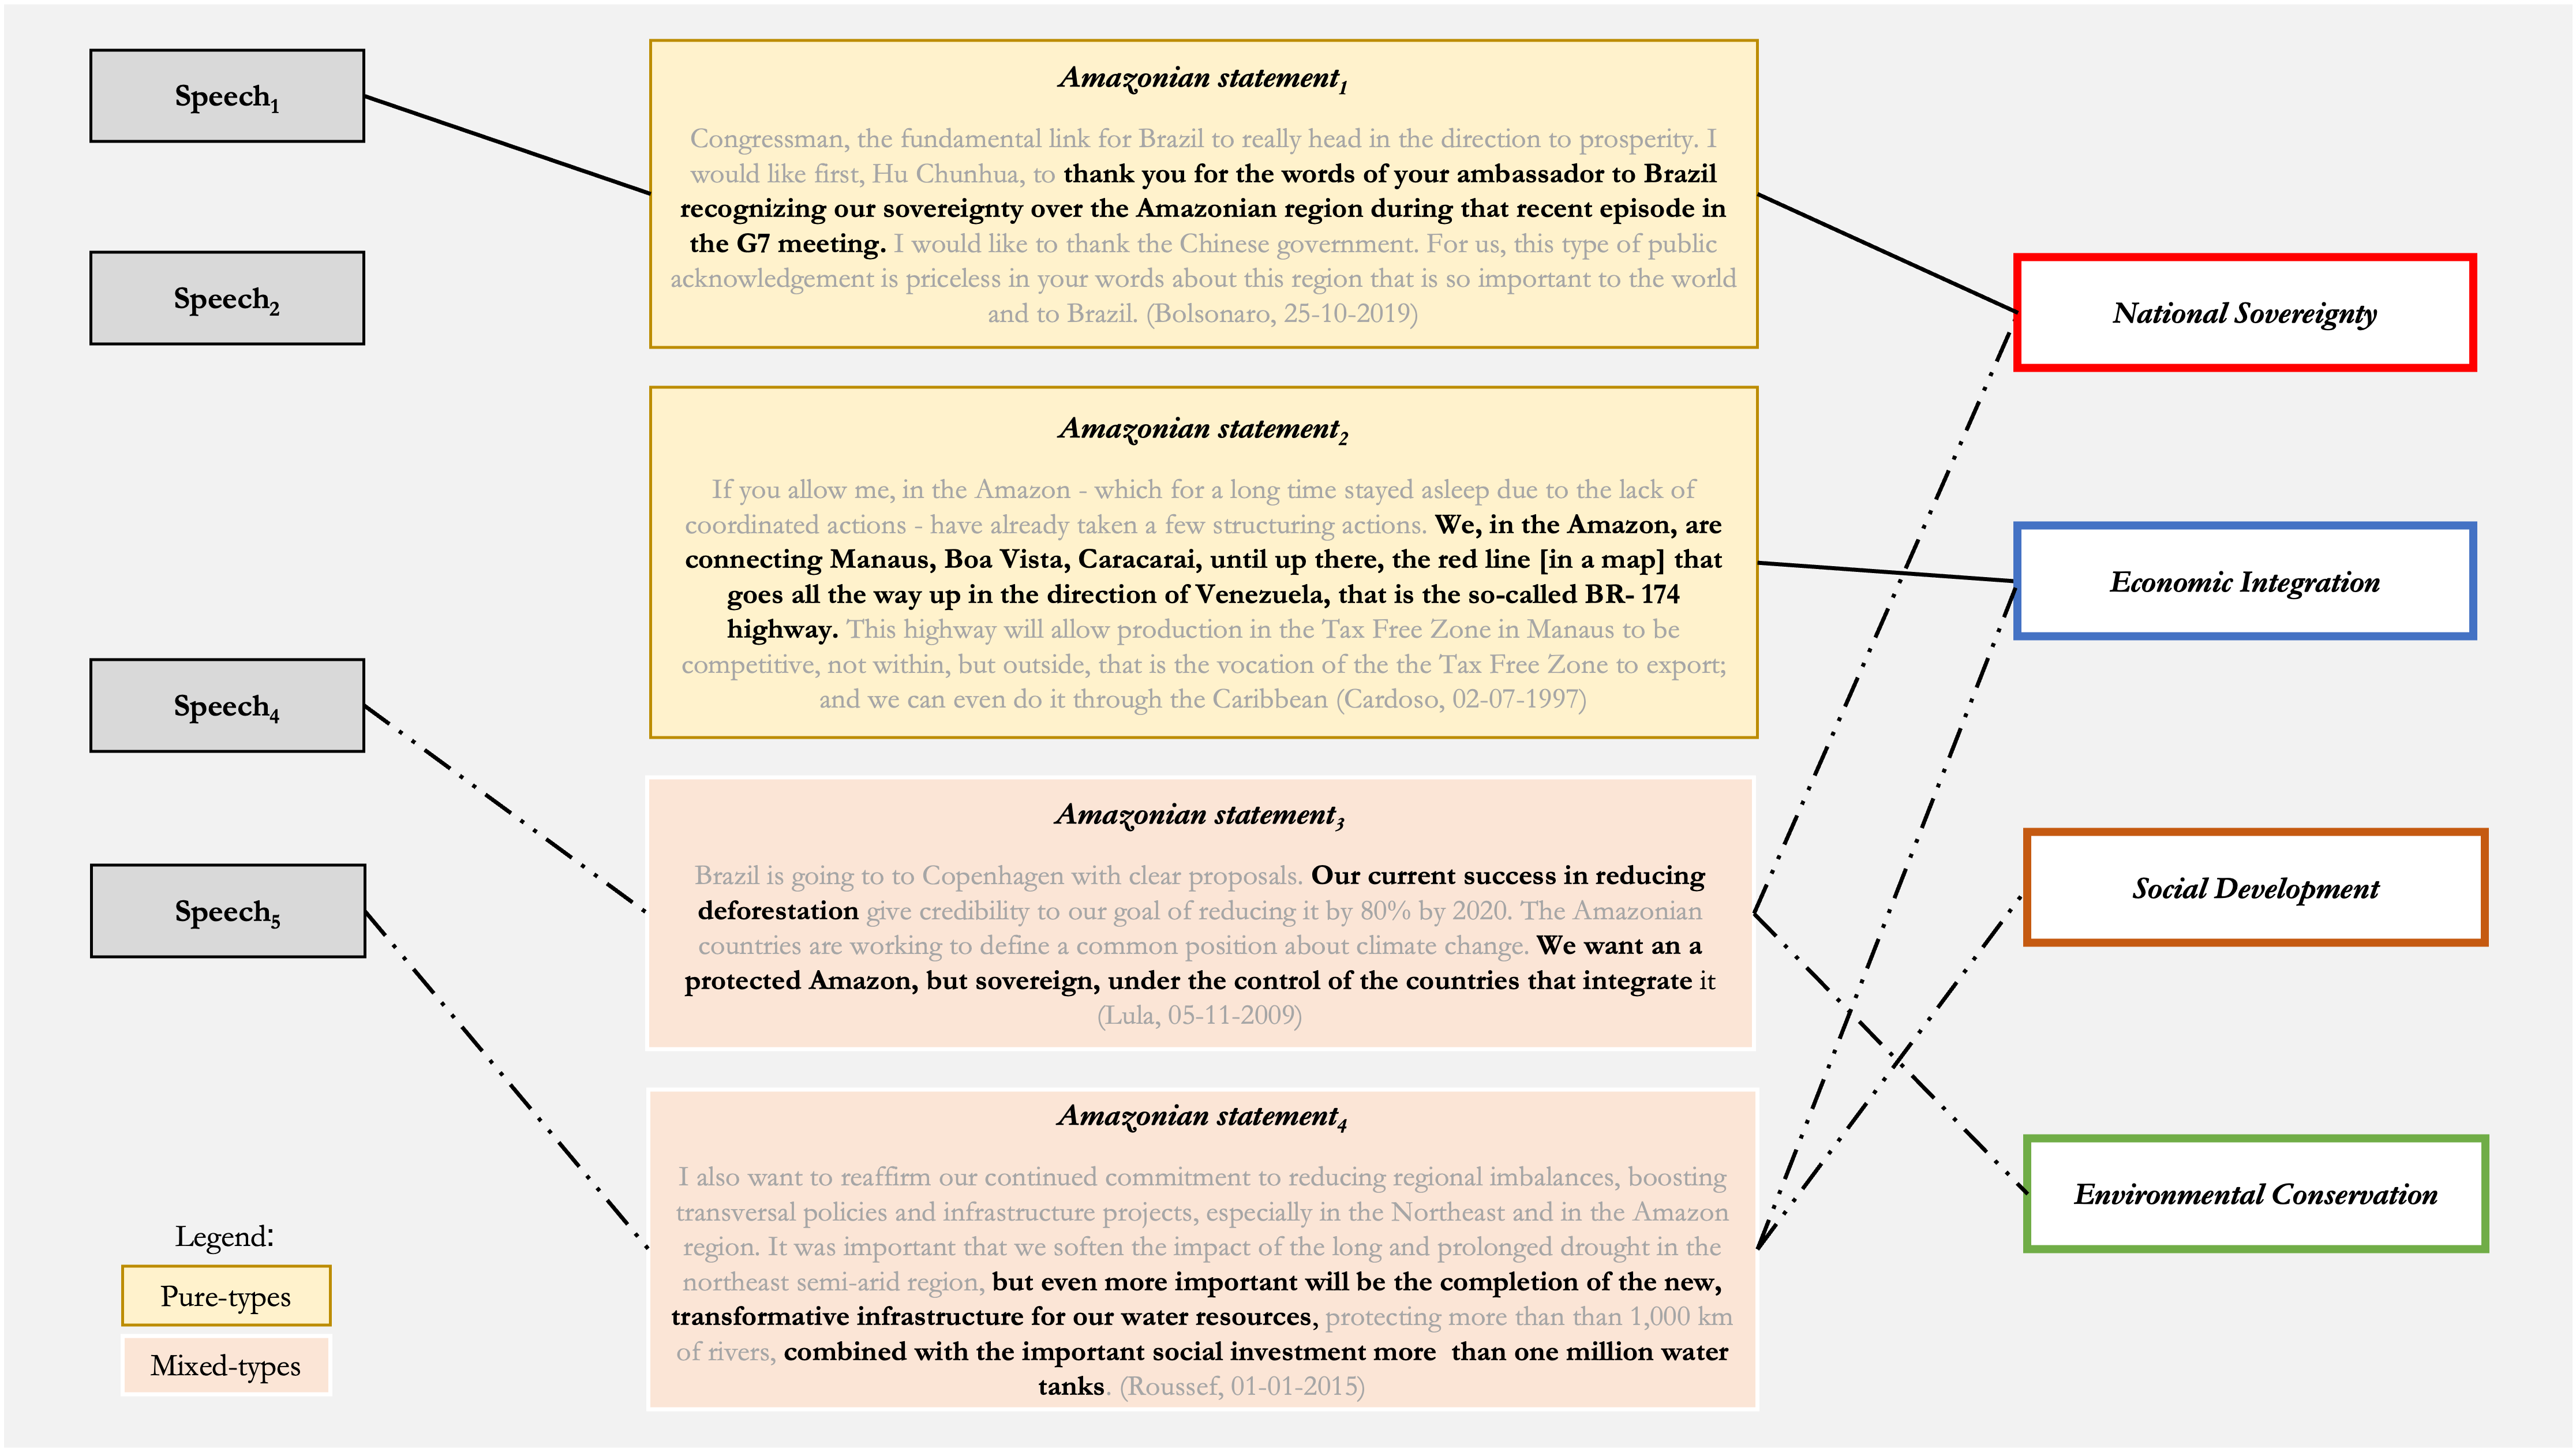
\includegraphics[width=1\linewidth]{figure1pic} \caption{Operationalization of problem-constructions}\label{fig:figure1}
\end{figure}

\end{landscape}

Second, with the codebook in hand, each one of the authors, separately,
hand-coded the same set of 1007 randomly selected Amazonian statements.
This amount refers to 50\% of all the Amazon Statements identified. We
chose to hand code half of the observations because there are several
nuances in discourse in how presidents talk about the Amazon over time
and as a problem.As the size of the training set should increase with
the number of categories (Grimmer, Roberts, and Stewart 2022), we deemed
four categories and 50\% of the statements as reliable. This allows a
robust validation set to verify the models. Also, automating the coding
of half of the observations saved the authors over one month of work in
comparison to manual coding. The intercoder agreement for hand-coded
categories was 85\%, on average. For each non-matching coded
observation, the co-authors discussed and sorted their disagreements.
Most disagreements related to different interpretations of the codebook,
which were subsequently clarified.

Third, the hand-coded data is then randomly divided into a training set,
containing 80\% of the hand-coded observations (806 observations), and a
validation set, containing the remaining 20\% of the hand-coded data
(201 observations). We chose to employ a support-vector machine (SVM)
algorithm, a non-probabilistic linear classifier that classifies
documents by assigning points in mapped space to maximize the gap
between binary categories, to label texts (Meyer et al. 2021; Noble
2006). The SVM model is trained using the hand-coded training set and
then employed to classify observations in the validation set. The
trained SVM model was, on average 82\%, accurate in classifying
observations in the validation set before being tuned. After the SVM
model is tuned, we use the model to automatically code the remaining
1007 Amazonian statements. The final dataset for analysis, excluding
false positive matches, contains 1895 coded Amazonian statements.

\hypertarget{analysis-and-limitations}{%
\subsection{3.2 Analysis and
Limitations}\label{analysis-and-limitations}}

To analyze our data, we first present a series of different plots on the
proportions of Amazonian statements and problem-constructions over time
and by presidents. To test whether problem-constructions depend on where
presidents speak, we run four separate logistic regressions. Each model
takes the share of a specific problem-construction versus all other
problem-constructions as their dependent variable. This means we try to
predict the probability of a president constructing the Amazon as an
issue of (1) environmental conservation, (2) economic integration, (3)
social development, and (4) national sovereignty, separately, and in
relation to the remaining three problem-constructions. Our main
independent variable is the distance (in kilometers) from the state or
country capital where the speech took place to Manaus (the capital of
the Amazonas State and centrally located in the region). The logic
behind this relates to presidents playing multi-level games. We expect
presidents to change how they construct the Amazon based on their
believes of audiences' expectations.We interpret the plots and model
considering multiple Amazon-related events and policies over the last 30
years, with the support of existing literature, and their correlations
with different presidents and locations.

This approach comes with limitations. Our codebook is developed using
specific Amazon-related vocabulary. For example, a statement will be
coded as economic integration if it is meaningful support for the
tax-free zone of Manaus or a dam in the Amazon. However, the economy is
generally a topic that presidents speak about frequently. Hence, the
high incidence of economic integration in Amazonian statements can also
be related to the higher importance of this problem-construction in
Brazil overall Moreover, we classify statements as Amazonian based on a
dictionary composed of a single lexicon stem: ``amazon''. We chose to do
so knowing that a few speeches about the Amazon might not contain the
lexicon ``Amazon'', for example, when the president says, ``the forest''
or ``deforestation''. Hence, we might be missing statements about Amazon
that do not refer to it. However, we consider this safer as we cannot be
sure that mentions of the forest or deforestation do not correspond to
other biomes such as the Cerrado or the Atlantic Forest. Finally, our
dataset covers only what is considered an official speech. Presidents,
though, give interviews, appear in debates, talk at campaign rallies,
and, more recently, post on social media. Problem-construction within
presidential discourse, thus, also happens in different sites for which
we do not account in this paper.

\hypertarget{how-has-the-amazon-been-constructed-as-a-problem}{%
\section{4 How has the Amazon been constructed as a
problem?}\label{how-has-the-amazon-been-constructed-as-a-problem}}

\hypertarget{the-rises-and-falls-of-the-amazon-as-a-topic-in-presidential-speeches}{%
\subsection{4.1 The rises and falls of the Amazon as a topic in
presidential
speeches}\label{the-rises-and-falls-of-the-amazon-as-a-topic-in-presidential-speeches}}

When, where, and how often do presidents speak about the Amazon? Figure
2, below, shows the proportion of speeches that mentions the Amazon in
relation to all speeches in a year. On average, presidents mention the
Amazon in 15.4\% of their speeches. For comparison purposes the averages
for other policy objects in the same corpus of speeches are: Inequality
(14.7\%), Criminality (17.3\%), Inflation (20.9\%), and Unemployment
(13.8\%). The frequency at which the Amazon appears across presidential
speeches inside, outside, and overall varies similarly across time (see
Figure 7 in appendix).

\begin{figure}
\centering
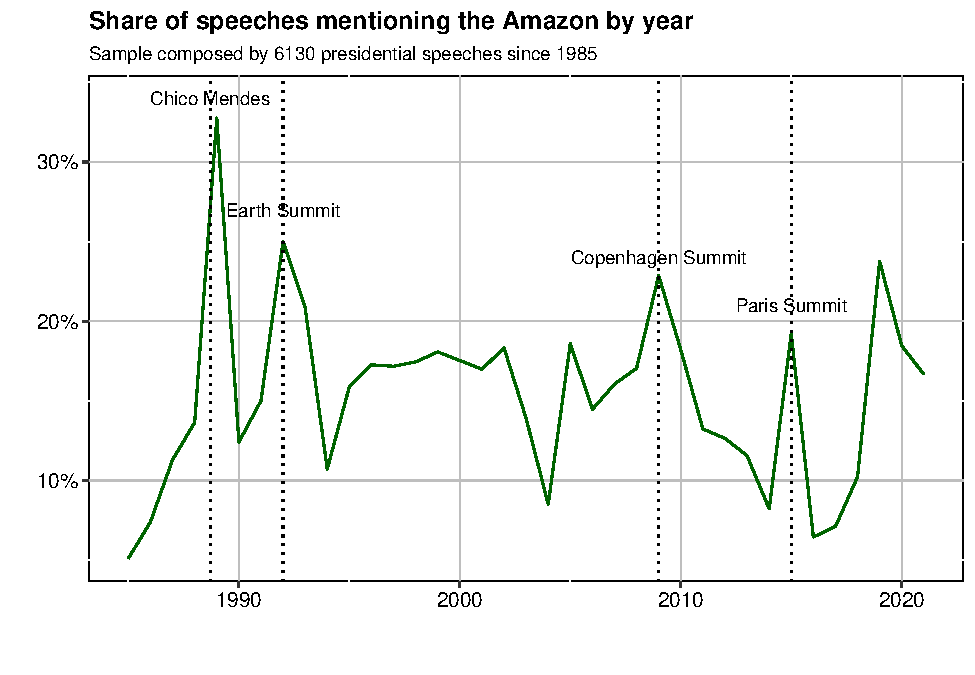
\includegraphics{Full_draft_20220901_files/figure-latex/Figure 2-1.pdf}
\caption{Amazonian speeches in time}
\end{figure}

We observe five local maxima both inside and outside Brazil: 1989, 1992,
2009, 2015, and 2019. These points coincide with internal and external
events that help us explain the rises and falls of the Amazon in
presidential discourse. From 1985 to 1988, the mentions of the Amazon in
official speeches increased from 4\% to 14\%. During this period, the
latest Brazilian Constitution was written, which gave indigenous and
traditional populations space to advocate for constitutional
environmental rights and the protection of their territories (S. B.
Hecht and Cockburn 1990). In 1989, however, the Amazon appeared in 32\%
of all speeches. This maximum correlates with the brutal murder of Chico
Mendes in the last days of 1988. The incident caught unprecedented
international attention and Sarney responded to this with a set of
policies to address deforestation (Capobianco 2021), including accepting
to host the 1992 Earth Summit (Keck and Sikkink 1998).

1990-91 the Amazon appeared in 12\% to 14\% of all speeches but, by
1992, this average increased to 25\%. The 1992 Earth Summit in Brazil
brought international attention to environmental topics related to the
Amazon. One of the big announcements, for example, was the consolidation
of the first transnational partnership for the Amazon, the G7 Pilot
Program, which brought a high number of financial resources to the
region for public policy implementation (Capobianco 2021). Throughout
the rest of the 1990s and 2000s, during the Cardoso (1995-2002) and Lula
administrations, the Amazon as a topic did not diverge much from the
average until 2009, when we see another maximum in mentions of the
Amazon. This coincides with the 2009 Copenhagen Summit and the steepest
decrease in deforestation rates since data is available as Figure 3,
below, illustrates. Lula led the delegation to Copenhagen with a
self-image of ``we do not promise, we deliver'' when the stakes about
climate change were high (Franchini and Viola 2019).

\begin{figure}
\centering
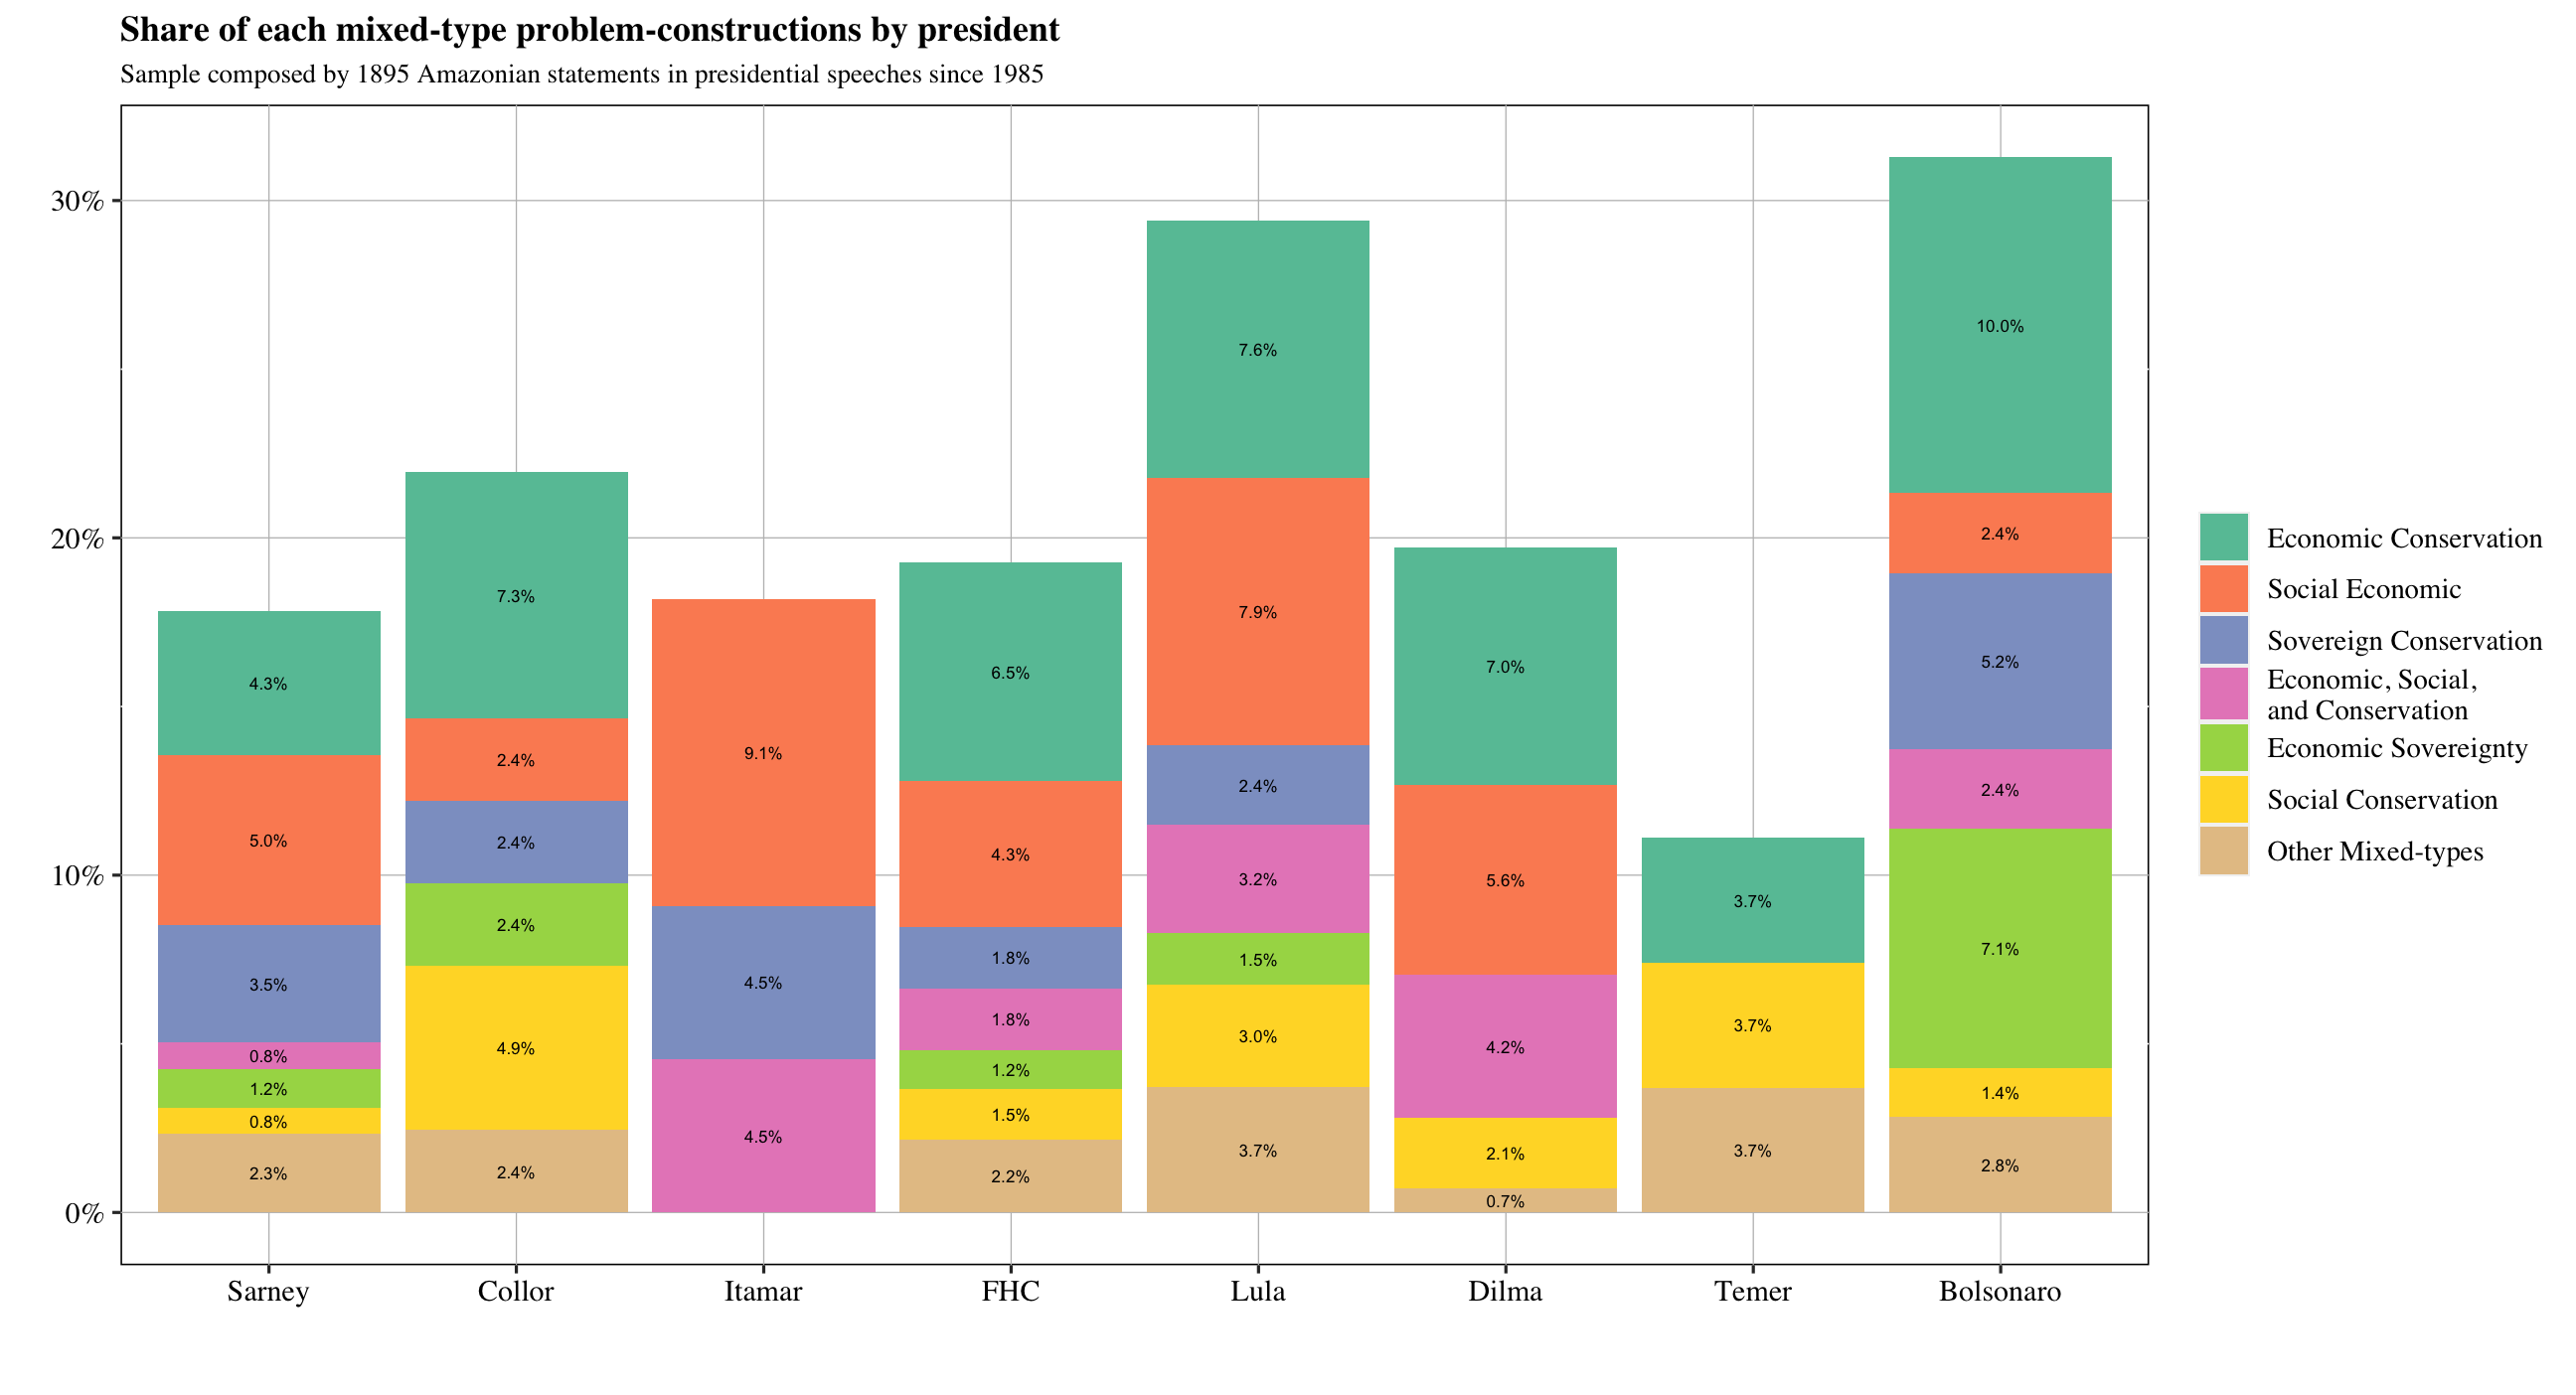
\includegraphics{Full_draft_20220901_files/figure-latex/Figure 3-1.pdf}
\caption{Deforestation rates since 1988}
\end{figure}

From 2010 to 2018, except for 2015, we see a general decrease in
mentions of the Amazon in all official presidential speeches. From 2010
to 2014, mentions of the Amazon went down from 18\% to 8\%.
Disagreements related to the priority of environmental preservation over
economic development were frequent, most notably in the case of approval
of the New Forest Code in 2012, which regularized land ownership of many
illegally deforested areas. The period was also marked by political and
economic instability which culminated in the impeachment of Rousseff in
2016. In 2015, the Amazon appeared in 19\% of all speeches. This maximum
coincides with the Paris summit which became a key turn in climate
politics after the failures of Copenhagen. Brazil went to the Paris
Summit with deforestation numbers slightly higher than Copenhagen and a
perception that there was a turn towards less conservation inside the
country. By 2016 mentions of Amazon in official speeches went down to
6\%, the lowest share since 1985.

We subsequently observe a steady increase from 6\% in 2016 to 24\% in
2019, the first year of Bolsonaro's presidency. At the time,
international and national media brought unprecedented attention to
Brazilian environmental issues as the record burning of the Amazon led
up to a red sky afternoon in São Paulo in August 2019. Alongside this,
Bolsonaro's dismantling of environmental governance and the threats to
leave the Paris Agreement had strong media attention, and, as a
response, the topic became prominent in his speeches. Bolsonaro went on
to retrieve Brazil's hosting status for COP25.

The frequency at which the Amazon appears in domestic and international
speeches varies in similar ways as the maxima in the topic frequencies,
led by the events discussed above, appear within and outside Brazil (see
Figure 7 appendix). We interpret this as evidence that relevant events
drive interest and alter how pressing the Amazon as a policy object is
perceived both nationally and internationally. This does not mean,
though, that when presidents speak about the Amazon, they highlight the
same issues.

\hypertarget{problem-constructions-in-time}{%
\subsection{4.2 Problem-constructions in
time}\label{problem-constructions-in-time}}

Our subsequent analysis of pure-types and mixed-types suggests that
governments do not defend a specific view of the Amazon. The same
governments construct the Amazon as various pure and mixed type
problems, which unravels a less cohesive story than that told by the
literature scrutinizing policy cycles.

\hypertarget{pure-type-problem-constructions}{%
\subsubsection{Pure-type
problem-constructions}\label{pure-type-problem-constructions}}

We conceptualize four problem-constructions: sovereignty, economic
integration, social development, and conservation. Figure 4, below,
illustrates the share of each pure-type in time. Pure
problem-constructions dominate, with an average of 56\% of all Amazonian
statements across time.We identify a discursive shift in
problem-constructions from developing the Amazon economically, to
conserving it and providing services to its citizens. Pure economic
integration constructions dominated constructions from 1985 to the late
2000s. This is especially pertinent during the Cardoso administration.
Brazilian presidents after Cardoso moved from employing one
problem-constructions consistently to a more diverse strategy. During
Lula's terms in office, constructing the Amazon purely as an issue of
economic integration decreased, while constructing the Amazon issues of
environmental conservation and social development increased.
Conservation and social development constructions surpassed economic
integration around 2010 and continued to dominate as Amazonian
constructions during Rousseff's administration. Still, environmental
conservation and social development problem-constructions were not as
dominant in terms of frequency or periods in time in discourses as
economic integration was until the early 2000s. Finally, we observe a
steady increase in sovereignty constructions in the late 2000s, reaching
the highest frequencies with the presidencies of Bolsonaro. As we
conceptualize and operationalize sovereignty as containing internal and
external perceived threats to the Amazon, we interpret this increase as
not only attacks on international interference in the Amazon but also on
indigenous and traditional populations.

\begin{figure}
\centering
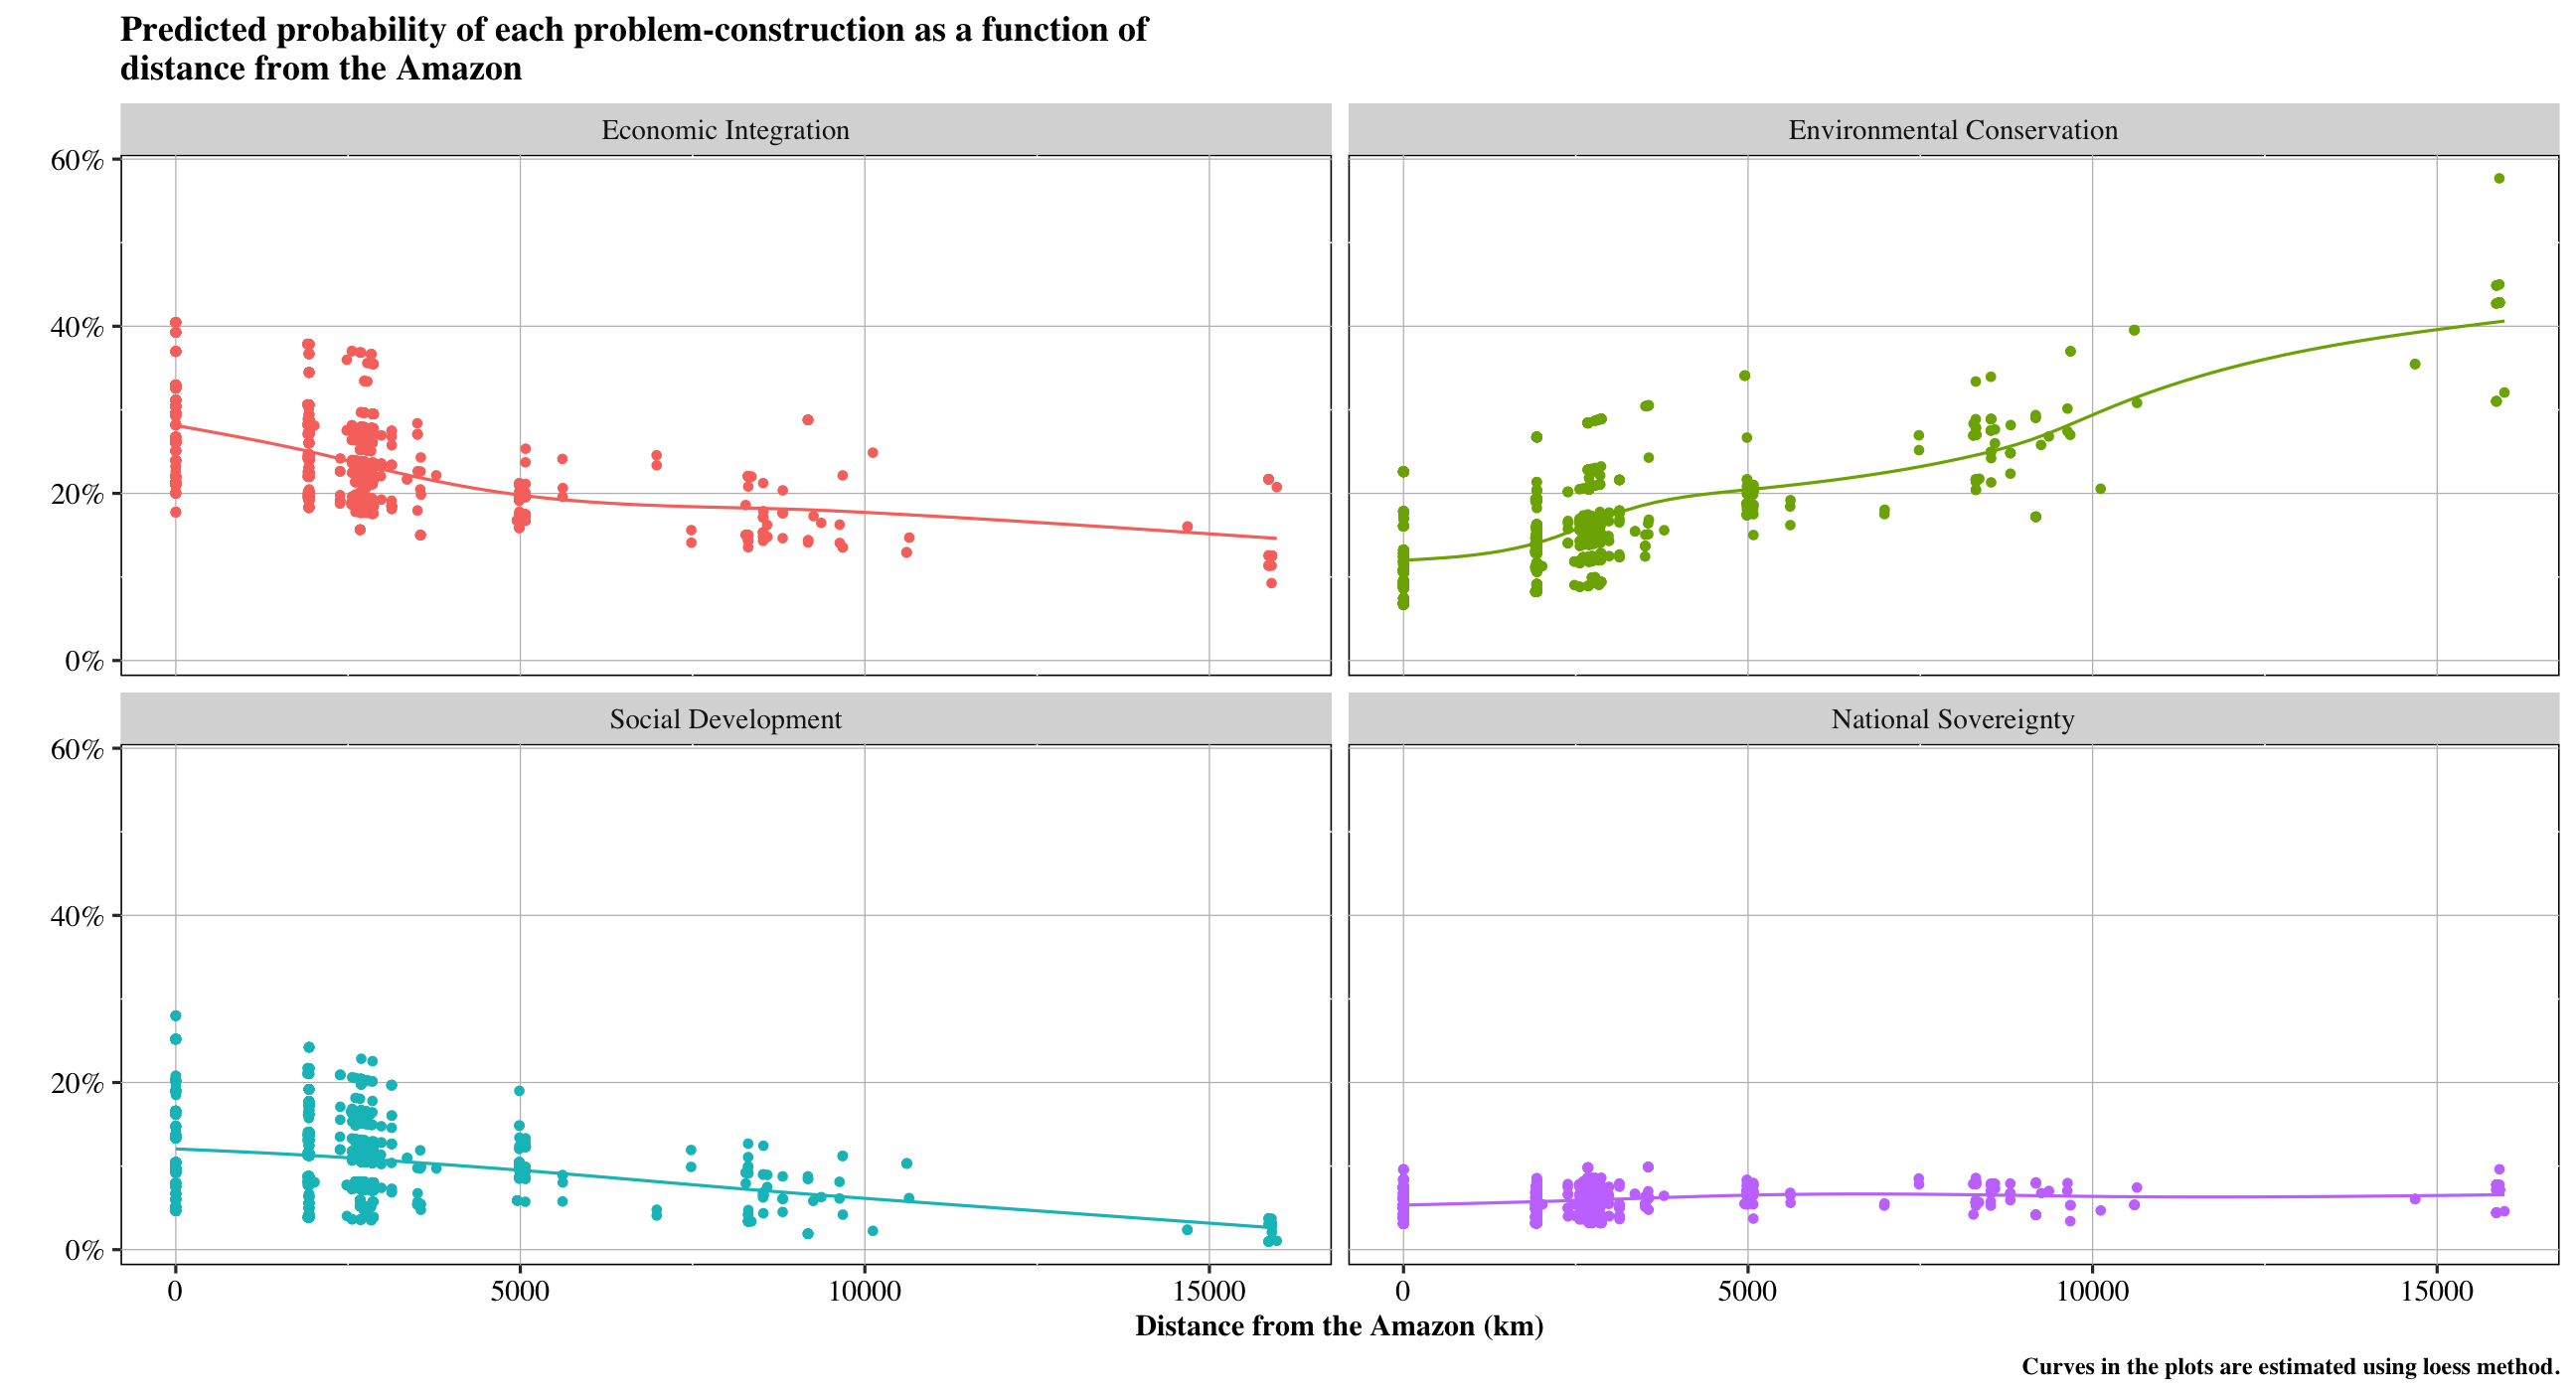
\includegraphics{Full_draft_20220901_files/figure-latex/Figure 4-1.pdf}
\caption{Pure-types in time}
\end{figure}

The trends identified are especially interesting considering Amazonian
policies and deforestation rates portrayed in Figure 3, above. First,
deforestation rates have a strong negative correlation with
environmental conservation. When deforestation rates increased from 1988
to 2004, and from 2012 until 2021, environmental conservation
constructions decreased. As deforestation rates decreased from 2004 to
2012, environmental conservation constructions in presidential speeches
increased. Capobianco (2021) argues that the unprecedented decrease in
deforestation we observed from 2004 to 2012 was a product of an increase
in the perception of stronger federal policies and police presence in
the Amazon region which, in turn, engendered a perception of a higher
risk of being caught and fined for deforestation. The shift from
constructing the Amazon as an issue of economic integration to an issue
of environmental conservation generates a perception that illegal
deforestation will be increasingly monitored and sanctioned. Second and
relatedly, deforestation rates have a positive and strong correlation
with economic integration. When deforestation increased from 1988 to
2004 and from 2012 to 2021, so did mentions to economic integration.
When deforestation decreased from 2004 to 2012, economic integration
decreased as well. This suggests that presidents might boast policy
outcomes related to economic integration as justifications for
deforestation.

\hypertarget{mixed-type-problem-constructions}{%
\subsubsection{Mixed-type
problem-constructions}\label{mixed-type-problem-constructions}}

In a speech, presidents might mix multiple problem-constructions within
a same statement about the Amazon. Although presidents prefer pure
problem-constructions, they also construct the Amazon as a multifaceted
issue. Mixed-type problem-constructions in discourse offer more
intricate understandings of the Amazon as a problem. Constructing the
Amazon as multiple issues averages at 18\% of all constructions in time.
Some mixed-types rarely appear so we focus our discussion on those
mixed-types with higher incidence. Figure 5, below, displays the
averages of mixed-types constructions by presidents.

\begin{figure}
\centering
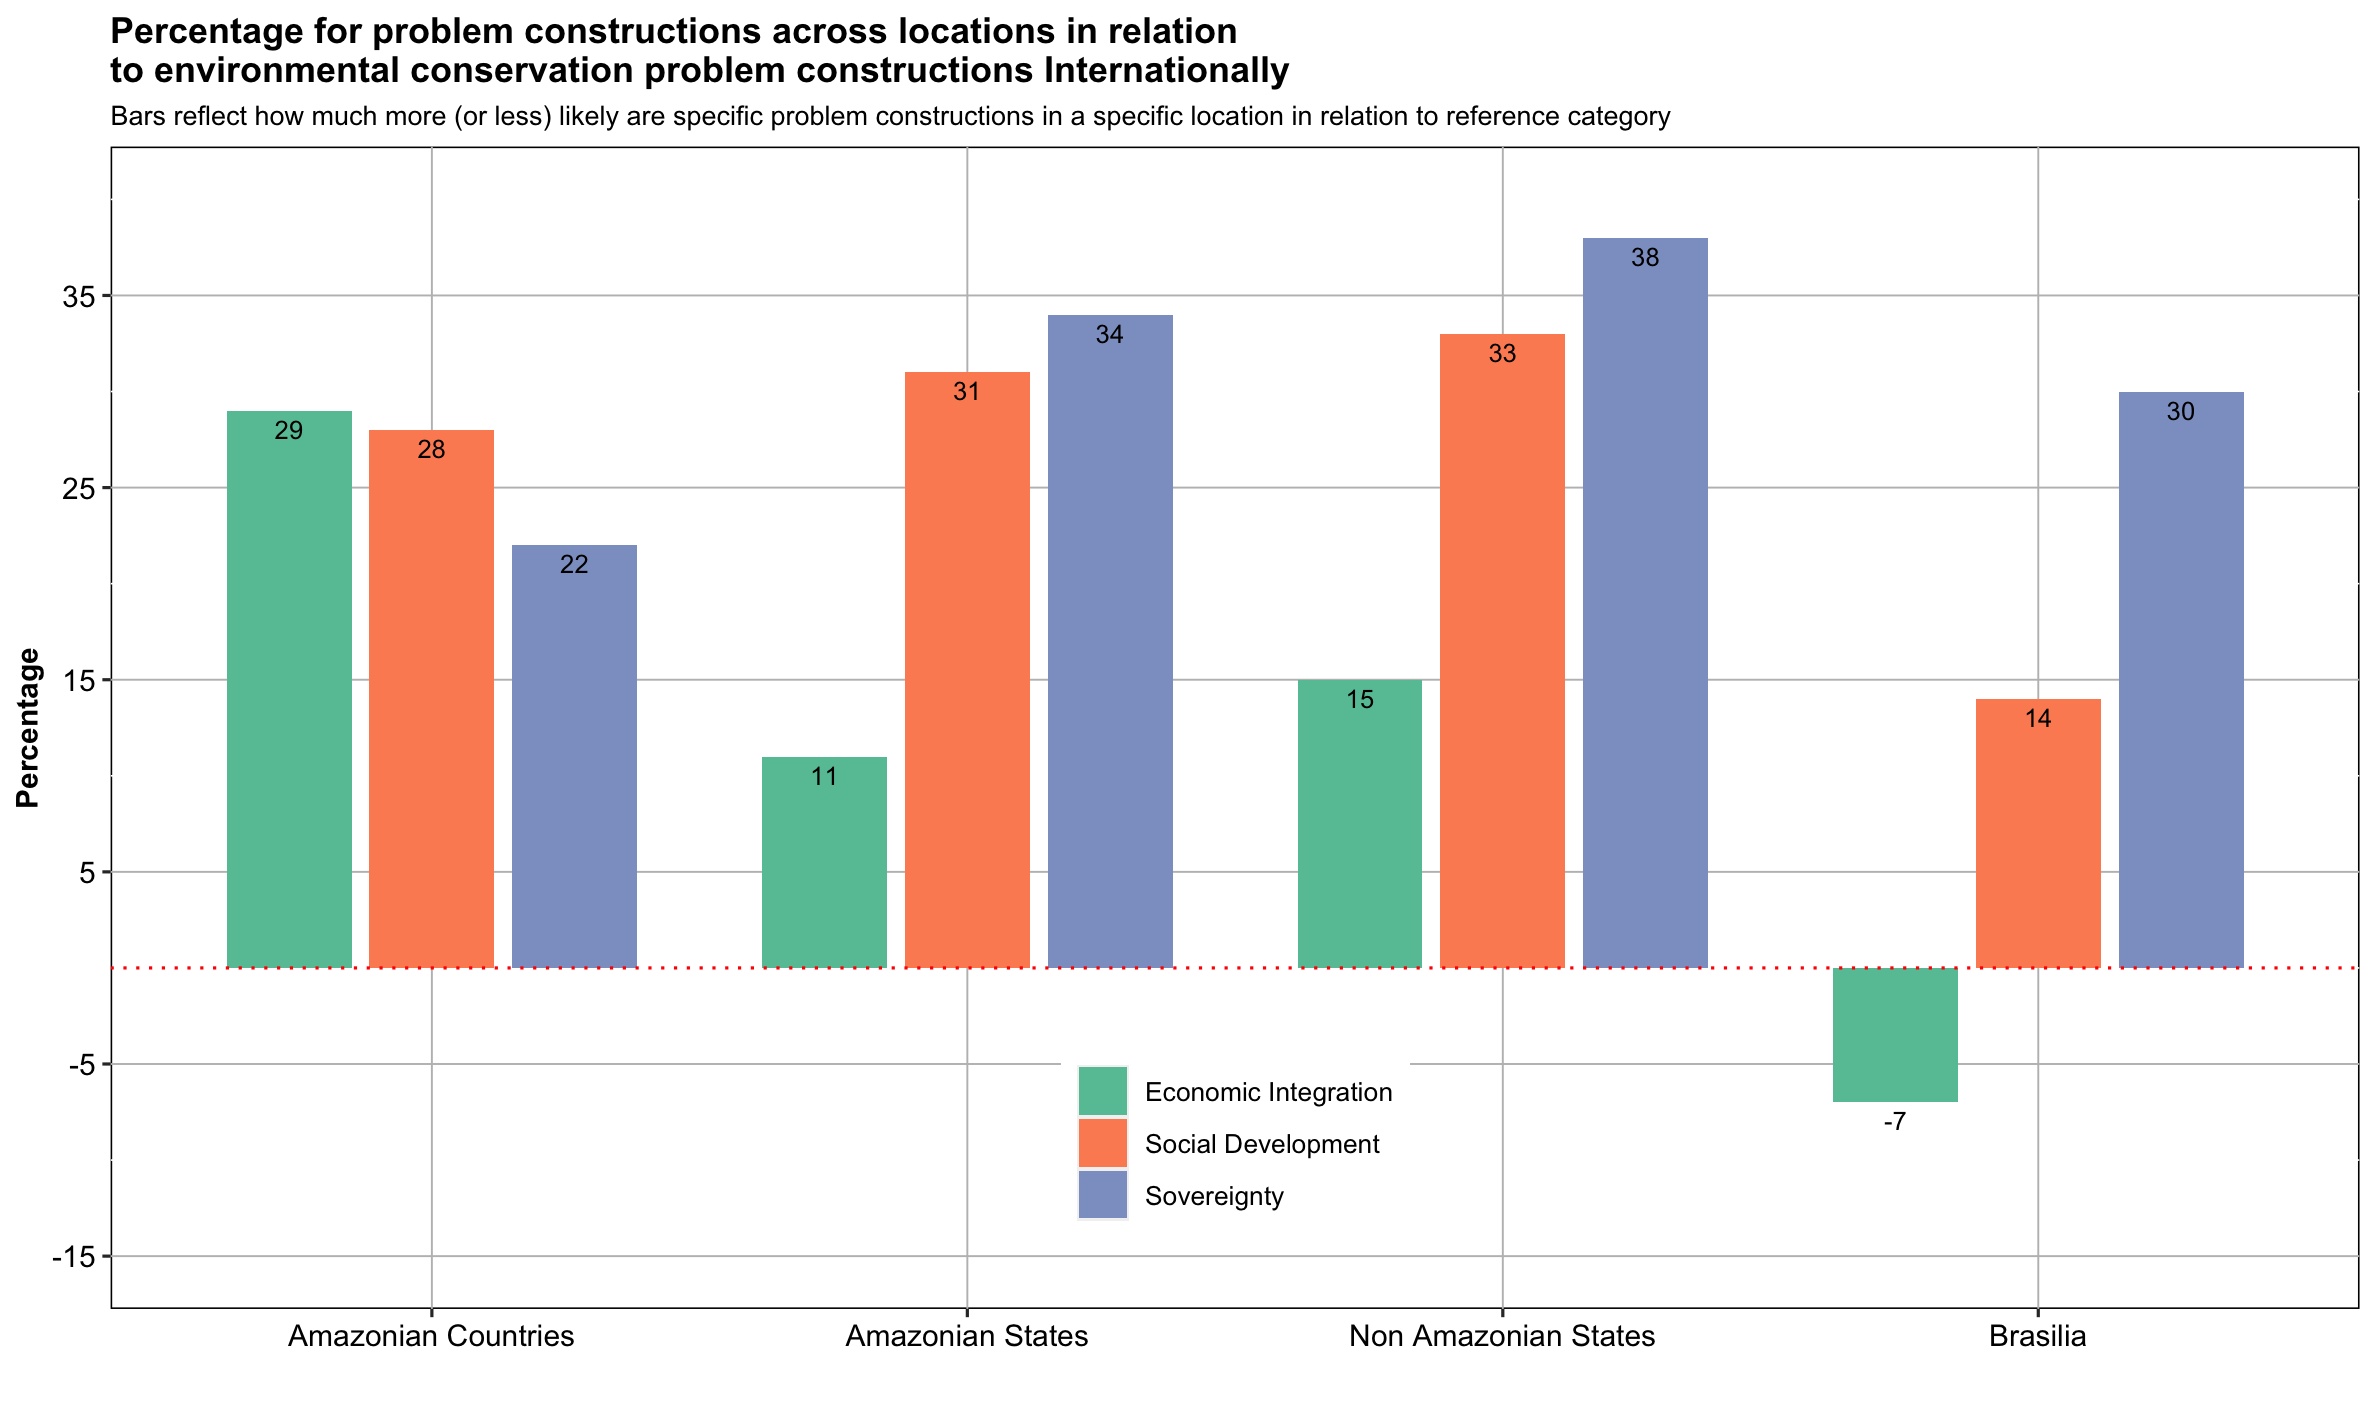
\includegraphics{Full_draft_20220901_files/figure-latex/Figure 5-1.pdf}
\caption{Mixed-types by president}
\end{figure}

The most frequent mixed-type problem construction of the Amazon is
economic conservation. This mixed-type construction, composed of
Amazonian statements that construct the Amazon as a problem of both
economic integration and environmental conservation, generally increased
over time. This increase suggests that later presidents, along with
being more diverse in how they construct the Amazon as an issue (see
Figure 4), increasingly find ways to reconcile the dictum between the
economy and the environment that had prevailed in the previous years.
The second most common mixed-type mixes social development and economic
integration and appears, on average, in 5.4\% of all statements. This is
not surprising, as developing countries like Brazil repeatedly claim a
``right to develop'', when it comes to negotiating strong climate
commitments and policies with a focus on both social development and
economic integration. Nonetheless, there is a general increase of
mixed-types over time, which is expected given the rise of global
agendas understanding interconnections of social, environmental, and
economic domains such as the Millennium Development Goals and the
Sustainable Development Goals.

Both Lula and Bolsonaro construct the Amazon as a multifaceted issue
more frequently than other presidents. Lula usually mixed economic
integration with environmental conservation and social development when
constructing the Amazon as an issue, while Bolsonaro constructs the
Amazon as an issue of national sovereignty and economic integration much
more than any other president, mimicking the military dictatorship
discourses and policies toward the region (S. B. Hecht and Cockburn
1990).

\hypertarget{the-amazonian-multi-level-game-boasting-policy-outside-and-talking-to-people-inside}{%
\subsection{4.3 The Amazonian multi-level game: boasting policy outside
and talking to people
inside}\label{the-amazonian-multi-level-game-boasting-policy-outside-and-talking-to-people-inside}}

The Amazon region, forests, and peoples have historically been the topic
of local, national, and international debates. This implies that
audiences' priorities in each setting change and consequently which
policies are appropriate to solve the ``Amazon issue'' differ as well.
As presidents physically move farther away from the Amazon, audiences
might have different stakes and interests in it. While speeches inside
the Amazon might focus on social development, for example, speeches in
the United Nations in New York might highlight environmental
conservation. To investigate the relationship between where presidents
speak and how they construct the Amazon as an issue, we run four
logistic regressions, one for each pure-type construction as a dependent
variable. We focus on pure-type constructions as these represent most
constructions and avoid ambiguity. The independent variable for all
models is the distance between the state country capital to Manaus.
Figure 6, below, depicts the predicted probabilities from the models
(see Table 1) as functions of distance.

\begin{figure}
\centering
\includegraphics{Full_draft_20220901_files/figure-latex/Figure 6-1.pdf}
\caption{Logistic Regression predicted values}
\end{figure}

We convert log odds from Table 1, below, into probabilities \footnote{See
  table 3 in appendix for all odds ratios and confidence intervals.}. It
shows that for each 1000Km increase, we find an increase of 52.8\% in
the predicted probability of constructing the Amazon as an issue of
environmental preservation. That is, the farthest away the president is
from the Amazon region, the more likely the president is to construct it
as an issue of environmental conservation. Second,the opposite is true
for both economic integration (and social development): for an increase
of 1000Km, we find a decrease of 48.5\% (47.4\%), respectively. When
speaking within the Amazon, presidents focus on social development and
economic integration. This entails that conservation might be a
desirable construction when speaking internationally about the Amazon,
but not at the local level, where presidents highlight economic and
social development. This multi-level game implies that presidents talk
to the economic and social needs of the people domestically while
boasting about environmentalism internationally. Finally, national
sovereignty problem constructions do not appear to change with distance.

\begin{landscape}


% Table created by stargazer v.5.2.3 by Marek Hlavac, Social Policy Institute. E-mail: marek.hlavac at gmail.com
% Date and time: Tue, Sep 20, 2022 - 16:35:39
\begin{table}[!htbp] \centering 
  \caption{Logistic Regressions Output} 
  \label{} 
\begin{tabular}{@{\extracolsep{5pt}}lcccc} 
\\[-1.8ex]\hline 
\hline \\[-1.8ex] 
 & \multicolumn{4}{c}{\textit{Dependent variable:}} \\ 
\cline{2-5} 
\\[-1.8ex] & Conservation & Economic Integration & Social Development & Sovereignty \\ 
\\[-1.8ex] & (1) & (2) & (3) & (4)\\ 
\hline \\[-1.8ex] 
 Distance from the Amazon in 1000s of km & 0.115554$^{***}$ & $-$0.056590$^{**}$ & $-$0.101285$^{**}$ & 0.009384 \\ 
  & (0.021453) & (0.023979) & (0.039849) & (0.038080) \\ 
  Election year & 0.287908$^{*}$ & $-$0.022328 & 0.328917$^{*}$ & $-$0.448696$^{*}$ \\ 
  & (0.156660) & (0.132762) & (0.171163) & (0.269325) \\ 
  Yearly Deforestation & $-$0.031739$^{***}$ & 0.040870$^{***}$ & $-$0.072349$^{***}$ & $-$0.031859$^{*}$ \\ 
  & (0.011298) & (0.008404) & (0.013232) & (0.016768) \\ 
  Yearly   Inflation & 0.000387$^{***}$ & $-$0.000231$^{**}$ & $-$0.000205 & 0.000215 \\ 
  & (0.000104) & (0.000104) & (0.000151) & (0.000177) \\ 
  Constant & $-$1.718459$^{***}$ & $-$1.568837$^{***}$ & $-$0.909845$^{***}$ & $-$2.300558$^{***}$ \\ 
  & (0.190667) & (0.159988) & (0.213791) & (0.280849) \\ 
 \hline \\[-1.8ex] 
Observations & 1,842 & 1,842 & 1,842 & 1,842 \\ 
Log Likelihood & $-$748.648200 & $-$1,022.790000 & $-$620.264400 & $-$399.290500 \\ 
Akaike Inf. Crit. & 1,507.296000 & 2,055.579000 & 1,250.529000 & 808.581000 \\ 
\hline 
\hline \\[-1.8ex] 
\textit{Note:}  & \multicolumn{4}{r}{$^{*}$p$<$0.1; $^{**}$p$<$0.05; $^{***}$p$<$0.01} \\ 
\end{tabular} 
\end{table} 

\end{landscape}

Our models also suggest that deforestation plays an important role.
Presidents are, for example, more likely to construct the Amazon as an
issue of environmental conservation as deforestation decreases.
Alternatively, as deforestation increases, presidents are more likely to
construct the amazon as an issue of economic integration. This indicates
that Brazil created a self-image of a strong climate leadership because
of the good results achieved from 2004 to 2012 (Franchini and Viola
2019). In the same fashion, economic integration problem-constructions
are likely deployed as a justification for increasing deforestation
rates.

\hypertarget{discussion-and-conclusion}{%
\section{5 Discussion and Conclusion}\label{discussion-and-conclusion}}

This paper investigates how the Brazilian Amazon has been constructed as
a problem in Brazilian presidential speeches since 1985. Our findings
are threefold: we find that the frequency of the Amazon as a topic in
speeches inside and outside Brazil is equally driven by domestic events
(e.g.~the assassination of Chico Mendes) as well as international events
(Climate Summits). Second, the same government adopts a diverse range of
problem-construction. While economic integration dominated discourse
from 1985 to the mid-2000s, environmental conservation and social
development constructions steadily grew in the 2000s, temporarily
surpassing economic integration as a more common problem-construction
from 2010 to 2015. This implies an overall movement from only exploiting
the Amazon for economic purposes to exploiting it and protecting it.
Constructing the Amazon as an issue of sovereignty became more pertinent
after 2010. Finally, we find that presidents are more likely to
construct the Amazon as an environmental conservation problem than
economic integration or social development, as presidents move away from
the Amazon region. Conceptually, this contributes to understanding the
social construction of the Amazon in discourses and how these relate to
policies and environmental outcomes. Empirically, we provide the first
comprehensive overview of when, where, and how the Amazon is constructed
as an issue in presidential discourse.

Discursive problem-construction within democracies legitimizes ways of
thinking and acting towards the environment. If presidents promote an
agenda of economic and social development within Brazil that diverges
from the one promoted outside of Brazil, to what extent does the
implemented agenda respond to domestic versus international demands? The
Brazilian government successfully funded domestic public policy with
transnational support on several occasions: the 1992 Pilot Programme of
the G7 for the Protection of Rainforest; the 2001 Amazon Regional
Protected Areas Program by the World Bank and others; and the 2008
Amazon Fund which provided over USD 1 billion (Silva-Muller and Faul
2022). Concurrently, the national agenda of economic integration or
social development was pursued. For instance, rural credit offered to
local agricultural producers in Amazonian states, went up from 500
million reais a year in 1999 to over 4 billion a year by 2012
(Capobianco 2021). Multiple contradictory policies negotiated
simultaneously, imply that presidents construct policy objects as issues
important to local electorates within the Amazon while, at the same
time, highlighting aspects important for international actors elsewhere.

The decrease in deforestation that took place in Brazil from 2004 to
2012, was accompanied by a period of strong economic growth. With the
strengthening of environmentalism, through the participation of
indigenous and civil society in politics (Hochstetler and Keck 2007),
the fall of economic integration problem-construction and the rise of
both social development and environmental conservation constructions in
the 2000s suggest a new balance between granting local livelihoods their
rights and economic development. This new balance was both unprecedented
and not long-standing. Unprecedented because never before the
environment and people were equally present as the economy in
presidential discourse. Not long-standing because the dismantling of
environmental policy in favor of infrastructure and agricultural
expansion was already on its way in the late 2010s. The 2012 New Forest
Code is seen as a turning point: political opposition to conservation
organized itself and managed to lobby with the executive and won these
battles even though they were largely opposed by environmentalists.

The steady increase of sovereignty problem-constructions starting in
2010 brings an eerie twist. The embryo of Bolsonaro's Amazonian
discourse was breeding half a decade before he took office. Bolsonaro is
a product of political re-organization of national and international
actors - to which Rousseff and Temer were already responding in
discourse - rather than the cause of change in politics. The political
forces in Brazilian democracy that drove these policy and discursive
changes in problem-construction were long in the making, Bolsonaro's
problem-constructions and policies are the strongest forms of this
shift.

\hypertarget{acknowledgements}{%
\section{Acknowledgements}\label{acknowledgements}}

The authors are extremely grateful to Matias López, Graziella Moraes
Silva, and James Hollway for their support. The authors would also like
to thank Mario, Federico, Rodrigo, and Anna for valuable comments on
earlier drafts of this paper.

\hypertarget{disclosure-statement}{%
\section{Disclosure Statement}\label{disclosure-statement}}

The authors report there are no competing interests to declare.

\hypertarget{references}{%
\section{References}\label{references}}

\hypertarget{refs}{}
\begin{CSLReferences}{1}{0}
\leavevmode\vadjust pre{\hypertarget{ref-acker2021}{}}%
Acker, Antoine. 2021. {``Amazon Development,''} Oxford research
encyclopedia of latin american history.,.
\url{https://doi.org/10.1093/acrefore/9780199366439.013.837}.

\leavevmode\vadjust pre{\hypertarget{ref-aklin2020}{}}%
Aklin, Michaël, and Matto Mildenberger. 2020. {``Prisoners of the Wrong
Dilemma: Why Distributive Conflict, Not Collective Action, Characterizes
the Politics of Climate Change.''} \emph{Global Environmental Politics}
20 (4): 4--27. \url{https://doi.org/10.1162/glep_a_00578}.

\leavevmode\vadjust pre{\hypertarget{ref-alesina2009}{}}%
Alesina, Alberto F., and Paola Giuliano. 2009. {``Preferences for
Redistribution.''} \url{https://www.nber.org/papers/w14825}.

\leavevmode\vadjust pre{\hypertarget{ref-andonova2014}{}}%
Andonova, Liliana B. 2014. {``Boomerangs to Partnerships? Explaining
State Participation in Transnational Partnerships for Sustainability.''}
\emph{Comparative Political Studies} 47 (3): 481--515.
\url{https://doi.org/10.1177/0010414013509579}.

\leavevmode\vadjust pre{\hypertarget{ref-assuncao2015}{}}%
Assunção, Juliano, Clarissa Gandour, and Rudi Rocha. 2015.
{``Deforestation Slowdown in the Brazilian Amazon: Prices or
Policies?''} \emph{Environment and Development Economics} 20 (6):
697--722. \url{https://doi.org/10.1017/S1355770X15000078}.

\leavevmode\vadjust pre{\hypertarget{ref-bacchi2009}{}}%
Bacchi, Carol Lee. 2009. \emph{Analysing Policy: What's the Problem
Represented to Be?} Pearson.

\leavevmode\vadjust pre{\hypertarget{ref-barros2020}{}}%
Barros, Antonio Teixeira de. 2020. {``Discursos parlamentares sobre a
Amazônia: sobre o que falam os deputados brasileiros.''} \emph{Política
\& Sociedade} 19 (46): 299--331.
\url{https://doi.org/10.5007/2175-7984.2020.e66962}.

\leavevmode\vadjust pre{\hypertarget{ref-becker2005}{}}%
Becker, Bertha K. 2005. {``Geopolítica da Amazônia.''} \emph{Estudos
Avançados} 19 (April): 71--86.
\url{https://doi.org/10.1590/S0103-40142005000100005}.

\leavevmode\vadjust pre{\hypertarget{ref-bevitori2015}{}}%
Bevitori, Cinzia. 2015. {``Discursive Constructions of the Environment
in American Presidential Speeches 1960{\textendash}2013: A Diachronic
Corpus-Assisted Study.''} \emph{Corpora and Discourse Studies}, 110--33.
\url{https://doi.org/10.1057/9781137431738_6}.

\leavevmode\vadjust pre{\hypertarget{ref-brice2021}{}}%
Brice, and Smith. 2021. {``The Amazon Is Fast Approaching a Point of No
Return.''} \emph{Bloomberg.com}, July.
\url{https://www.bloomberg.com/news/features/2021-07-29/amazon-rainforest-deforestation-land-grabs-surge-under-bolsonaro-in-brazil}.

\leavevmode\vadjust pre{\hypertarget{ref-calderwood2019}{}}%
Calderwood, Kevin J. 2019. {``Discourse in the Balance: American
Presidential Discourse about Climate Change.''} \emph{Communication
Studies} 70 (2): 235--52.
\url{https://doi.org/10.1080/10510974.2019.1572636}.

\leavevmode\vadjust pre{\hypertarget{ref-calderwood2020}{}}%
---------. 2020. {``Going Global: Climate Change Discourse in
Presidential Communications.''} \emph{Environmental Communication} 14
(1): 52--67. \url{https://doi.org/10.1080/17524032.2019.1592005}.

\leavevmode\vadjust pre{\hypertarget{ref-campbell2015}{}}%
Campbell, Jeremy M. 2015. \emph{Conjuring Property: Speculation and
Environmental Futures in the Brazilian Amazon}. Illustrated edition.
Seattle: University of Washington Press.

\leavevmode\vadjust pre{\hypertarget{ref-capobianco2019}{}}%
Capobianco, João Paulo. 2019. {``Avances y retrocesos de la
sostenibilidad en la Amazonia: un análisis de la gobernanza
socioambiental en la Amazonia,''} January.
\url{https://gredos.usal.es/handle/10366/139311}.

\leavevmode\vadjust pre{\hypertarget{ref-capobianco2021}{}}%
---------. 2021. \emph{Amazônia: Uma Década de Esperança}. 1ª edição.
São Paulo: Estação Liberdade.

\leavevmode\vadjust pre{\hypertarget{ref-cezar2020}{}}%
Cezar, Rodrigo Fagundes. 2020. {``Brazilian Presidential Speeches from
1985 to July 2020.''}
\url{https://dataverse.harvard.edu/dataset.xhtml?persistentId=doi:10.7910/DVN/M9UU09}.

\leavevmode\vadjust pre{\hypertarget{ref-silva2019}{}}%
Da Silva, Antonio José Bacelar, and Erika Robb Larkins. 2019. {``The
Bolsonaro Election, Antiblackness, and Changing Race Relations in
Brazil.''} \emph{The Journal of Latin American and Caribbean
Anthropology} 24 (4): 893--913.

\leavevmode\vadjust pre{\hypertarget{ref-drummond2006}{}}%
Drummond, Jose, and Ana Flavia Barros-Platiau. 2006. {``Brazilian
Environmental Laws and Policies, 1934-2002: A Critical Overview.''}
\emph{Law and Policy} 28 (1): 83--108.
\url{https://doi.org/10.1111/j.1467-9930.2005.00218.x}.

\leavevmode\vadjust pre{\hypertarget{ref-franchini2019}{}}%
Franchini, Matias Alejandro, and Eduardo Viola. 2019. {``Myths and
Images in Global Climate Governance, Conceptualization and the Case of
Brazil (1989 - 2019).''} \emph{Revista Brasileira de Política
Internacional} 62 (September).
\url{https://doi.org/10.1590/0034-7329201900205}.

\leavevmode\vadjust pre{\hypertarget{ref-gillion2016}{}}%
Gillion, Daniel Q. 2016. \emph{Governing with Words: The Political
Dialogue on Race, Public Policy, and Inequality in America}. Cambridge:
Cambridge University Press.
\url{https://doi.org/10.1017/CBO9781316412299}.

\leavevmode\vadjust pre{\hypertarget{ref-grimmer2022}{}}%
Grimmer, Justin, Margaret E. Roberts, and Brandon M. Stewart. 2022.
\emph{Text as Data: A New Framework for Machine Learning and the Social
Sciences}. Princeton, New Jersey Oxford: Princeton University Press.

\leavevmode\vadjust pre{\hypertarget{ref-harris2021}{}}%
Harris, Bryan. 2021. {``Drought Puts Amazon at Risk of {`}Large-Scale
Dieback{'}, Researchers Warn.''} \emph{Financial Times}, July.
\url{https://www.ft.com/content/02071ae7-dcf5-4c61-9c3c-b55f5aef8b0e}.

\leavevmode\vadjust pre{\hypertarget{ref-hecht1990}{}}%
Hecht, Susanna B., and Alexander Cockburn. 1990. \emph{The Fate of the
Forest: Developers, Destroyers, and Defenders of the Amazon, Updated
Edition}. Chicago, IL: University of Chicago Press.
\url{https://press.uchicago.edu/ucp/books/book/chicago/F/bo10387801.html}.

\leavevmode\vadjust pre{\hypertarget{ref-hecht2020}{}}%
Hecht, Susanna, and Raoni Rajão. 2020. {``From {``}Green Hell{''} to
{``}Amazonia Legal{''}: Land Use Models and the Re-Imagination of the
Rainforest as a New Development Frontier.''} \emph{Land Use Policy} 96
(July): 103871. \url{https://doi.org/10.1016/j.landusepol.2019.02.030}.

\leavevmode\vadjust pre{\hypertarget{ref-hirschman1963}{}}%
Hirschman, Albert O. 1963. \emph{Journeys Toward Progress: Studies of
Economic Policy-Making in Latin America}. Twentieth Century Fund.

\leavevmode\vadjust pre{\hypertarget{ref-hirschman1975}{}}%
---------. 1975. {``Policymaking and Policy Analysis in Latin America: A
Return Journey.''} \emph{Policy Sciences} 6 (4): 385--402.
\url{https://www.jstor.org/stable/4531616}.

\leavevmode\vadjust pre{\hypertarget{ref-hochstetler2021}{}}%
Hochstetler, Kathryn. 2021. {``Climate Institutions in Brazil: Three
Decades of Building and Dismantling Climate Capacity.''}
\emph{Environmental Politics} 30 (sup1): 49--70.
\url{https://doi.org/10.1080/09644016.2021.1957614}.

\leavevmode\vadjust pre{\hypertarget{ref-hochstetler2007}{}}%
Hochstetler, Kathryn, and Margaret E. Keck. 2007. \emph{Greening Brazil:
Environmental Activism in State and Society}.
\url{https://doi.org/10.1215/9780822390596}.

\leavevmode\vadjust pre{\hypertarget{ref-keck1998}{}}%
Keck, Margaret E., and Kathryn Sikkink. 1998. \emph{Activists Beyond
Borders: Advocacy Networks in International Politics}. 1st Edition.
Ithaca, N.Y: Cornell University Press.

\leavevmode\vadjust pre{\hypertarget{ref-lopez2020}{}}%
López, Matias, Graziella Moraes Silva, Chana Teeger, and Pedro Marques.
2020. {``Economic and Cultural Determinants of Elite Attitudes Toward
Redistribution.''} \emph{Socio-Economic Review}, May.
\url{https://doi.org/10.1093/ser/mwaa015}.

\leavevmode\vadjust pre{\hypertarget{ref-meyer2021}{}}%
Meyer, David, Evgenia Dimitriadou, Kurt Hornik, Andreas Weingessel, and
Friedrich Leisch. 2021. \emph{E1071: Misc Functions of the Department of
Statistics, Probability Theory Group (Formerly: E1071), TU Wien}.
\url{https://CRAN.R-project.org/package=e1071}.

\leavevmode\vadjust pre{\hypertarget{ref-miranda2021}{}}%
Miranda, David. 2021. {``Bolsonaro{'}s 1,000km Amazon Railway Will Cause
Climate Chaos. It Must Be Stopped.''} \emph{The Guardian}, July.
\url{https://www.theguardian.com/commentisfree/2021/jul/28/bolsonaro-amazon-railway-climate-chaos-must-be-stopped}.

\leavevmode\vadjust pre{\hypertarget{ref-noble2006}{}}%
Noble, William S. 2006. {``What Is a Support Vector Machine?''}
\emph{Nature Biotechnology} 24 (12): 1565--67.

\leavevmode\vadjust pre{\hypertarget{ref-padua2012}{}}%
Pádua, José Augusto. 2012. {``Environmentalism in Brazil: A Historical
Perspective.''} \emph{A Companion to Global Environmental History} 1:
455--73.

\leavevmode\vadjust pre{\hypertarget{ref-pereira2021}{}}%
Pereira, Joana Castro, and Eduardo Viola. 2021. \emph{Climate Change and
Biodiversity Governance in the Amazon: At the Edge of Ecological
Collapse?} Routledge.

\leavevmode\vadjust pre{\hypertarget{ref-putnam1988}{}}%
Putnam, Robert D. 1988. {``Diplomacy and Domestic Politics: The Logic of
Two-Level Games.''} \emph{International Organization} 42 (3): 427--60.
\url{http://www.jstor.org/stable/2706785}.

\leavevmode\vadjust pre{\hypertarget{ref-rajao2020}{}}%
Rajão, Raoni, Britaldo Soares-Filho, Felipe Nunes, Jan Börner, Lilian
Machado, Débora Assis, Amanda Oliveira, et al. 2020. {``The Rotten
Apples of Brazil's Agribusiness.''} \emph{Science} 369 (6501): 246--48.
\url{https://doi.org/10.1126/science.aba6646}.

\leavevmode\vadjust pre{\hypertarget{ref-silva-muller2022a}{}}%
Silva-Muller, Livio. 2022. {``Payment for Ecosystem Services and the
Practices of Environmental Fieldworkers in Policy Implementation: The
Case of Bolsa Floresta in the Brazilian Amazon.''} \emph{Land Use
Policy} 120 (September): 106251.
\url{https://doi.org/10.1016/j.landusepol.2022.106251}.

\leavevmode\vadjust pre{\hypertarget{ref-silva-muller2022}{}}%
Silva-Muller, Livio, and Moira V. Faul. 2022. {``Protecting the Amazon
and Its People: The Role of Civil Society in Local Effectiveness of
Trasnational Partnerships.''} In \emph{Partnerships for Sustainability
in Contemporary Global Governance}, 83--103. Routledge.
\url{https://doi.org/10.4324/9781003148371-6}.

\leavevmode\vadjust pre{\hypertarget{ref-soares-filho2014}{}}%
Soares-Filho, Britaldo, Raoni Rajão, Marcia Macedo, Arnaldo Carneiro,
William Costa, Michael Coe, Hermann Rodrigues, and Ane Alencar. 2014.
{``Cracking Brazil's Forest Code.''} \emph{Science} 344 (6182): 363--64.
\url{https://doi.org/10.1126/science.1246663}.

\leavevmode\vadjust pre{\hypertarget{ref-sposito2021}{}}%
Sposito, Henrique. 2021. \emph{Poldis: Tools for Analyzing Political
Discourse}. \url{https://github.com/henriquesposito/poldis}.

\leavevmode\vadjust pre{\hypertarget{ref-viola1987}{}}%
Viola, Eduardo J. 1987. {``O Movimento Ecológico No Brasil, 1974-1986:
Do Ambientalismo à Ecopolítica.''} \emph{Revista Brasileira de Ciencias
Sociais} 3 (93): 5--26.
\url{http://anpocs.com/images/stories/RBCS/03/rbcs03_01.pdf}.

\leavevmode\vadjust pre{\hypertarget{ref-lepolaindewaroux2021}{}}%
Waroux, Yann de, Rachael D. Garrett, Mollie Chapman, Cecilie Friis,
Jeffrey Hoelle, Leonie Hodel, Kelly Hopping, and Julie Gwendolin
Zaehringer. 2021. {``The Role of Culture in Land System Science.''}
\emph{Journal of Land Use Science} 16 (4): 450--66.
\url{https://doi.org/10.1080/1747423X.2021.1950229}.

\leavevmode\vadjust pre{\hypertarget{ref-zarefsky2004}{}}%
Zarefsky, David. 2004. {``Presidential Rhetoric and the Power of
Definition.''} \emph{Presidential Studies Quarterly} 34 (3): 607--19.
\url{https://www.jstor.org/stable/27552615}.

\end{CSLReferences}

\newpage

\hypertarget{appendix}{%
\section{Appendix}\label{appendix}}

\begin{figure}
\centering
\includegraphics{Full_draft_20220901_files/figure-latex/Figure 7-1.pdf}
\caption{Amazonian speeches in time and space}
\end{figure}

\begin{landscape}

\begin{table}

\caption{\label{tab:codebook}Amazonian Problem-Construction Codebook}
\centering
\resizebox{\linewidth}{!}{
\fontsize{9}{11}\selectfont
\begin{tabu} to \linewidth {>{\raggedright\arraybackslash}p{3cm}>{\raggedright\arraybackslash}p{9cm}>{\raggedright\arraybackslash}p{9cm}}
\toprule
problem-construction & Description & Example\\
\midrule
\textbf{\cellcolor{gray!6}{National Sovereignty}} & \cellcolor{gray!6}{This code constructs the Amazon region and/or forest as an issue of national sovereignty. We understand claims of sovereignty as a particular problem-construction that touches on imaginaries of external threats to territory. Relatedly, we also understand sovereignty as raising concerns about wrong perspectives and criticism from foreign and non-state actors about government action related to the Brazilian Amazon. In all, it advances the view that the Amazon is Brazilian, foreign, and non-state presence in the region needs to be monitored closely.} & \cellcolor{gray!6}{Congressman, the fundamental link for Brazil to really head in the direction to prosperity. I would like first, Hu Chunhua,  to thank you for the words of your ambassador to Brazil recognizing our sovereignty over the Amazonian region during that recent episode in the G7 meeting. I would like to thank the Chinese government. For us, this type of public acknowledgement is priceless in your words about this region that is so important to the world and to Brazil. (Bolsonaro 25/10/2019)}\\
\textbf{Economic Integration} & This code constructs the Amazon region and/or forest as an issue of economic integration. It advances the view that the Amazon needs to be developed and connected to the national economy. This includes expanding the agricultural frontier through incentives, creating a diverse set of infrastructure (roads, dams, internet, radio, energy), fostering differing industries (tourism, mining, cattle, agriculture and so on) through tax-free zones, as well as facilitating the exploitation of natural resources for developmental purposes. & If you allow me, in the Amazon - which for a long time stayed asleep due to the lack of coordinated actions - have already taken a few structuring actions. We, in the Amazon, are connecting Manuas, Boa Vista, Caracarai, until up there, the red line [in a map] that goes all the way up in the direction of Venezuela, that is the so-called  BR-174 highway. This highway will allow production in the Tax Free Zone in Manaus to be competitive, not within, but outside, that is the vocation of the the Tax Free Zone to export; and we can even do it through the Caribbean (Cardoso 02/07/1997)\\
\textbf{\cellcolor{gray!6}{Social Development}} & \cellcolor{gray!6}{This code constructs the Amazon region and/or forest as an issue of social development. It advances the view that Amazon is full of citizens who should have their rights guaranteed. This refers to the construction of schools and universities (right to education), of hospitals (right to health), and of housing (right to house). This also includes guarantees of a dignified life with decent employment, access to water and sanitation, as well as access to electricity, internet, radio, and light. Finally, this includes referrals to culture and the right to vote.} & \cellcolor{gray!6}{The state does not work for profits, the state needs to guarantee dignity, we find that a citizen who lives in the riverside of the Amazon river, 600 kilometers from Manaus, has the right to have the electricity in their house, to owe a fridge, to owe a television where to watch the soap operas. We have invested over 14 billion reais in this program, in three and a half years. Do you know how many electrical lines we have already built? One million kilometers of lines. (Lula 20/11/2009)}\\
\textbf{Environmental Conservation} & This code constructs the Amazon region and/or forest as an issue of conservation. This problem-construction focuses on the value of a standing forest and of the preserved ecosystem in the region. The conservationist narrative advances the view that Amazon should be preserved, deforestation should be halted, and the practices of indigenous and traditional populations should be maintained and fostered. It advances the view that the emission of greenhouse gasses should be halted, that renewable energy should be supported, and that protected areas should be created. & I have put in place emergency measures, I have suspended the exports of wood logs, I have suspended the fiscal incentives and credits to projects that could damage the environment in the amazon and I have made a license mandatory to gold mining that prohibits utilizing mercury in the process. This began the restructuring of the governmental system of control and preservation of the environment, I have created the Brazilian Institute for the Environment and Natural Resources [IBAMA], which will be headed by Dr. Mesquita (Sarney 20/07/1989)\\
\bottomrule
\end{tabu}}
\end{table}

\end{landscape}

\begin{landscape}

<table style="border-collapse:collapse; border:none;">
<tr>
<th style="border-top: double; text-align:center; font-style:normal; font-weight:bold; padding:0.2cm;  text-align:left; ">&nbsp;</th>
<th colspan="3" style="border-top: double; text-align:center; font-style:normal; font-weight:bold; padding:0.2cm; ">con vs all</th>
<th colspan="3" style="border-top: double; text-align:center; font-style:normal; font-weight:bold; padding:0.2cm; ">EI vs all</th>
<th colspan="3" style="border-top: double; text-align:center; font-style:normal; font-weight:bold; padding:0.2cm; ">SD vs all</th>
<th colspan="3" style="border-top: double; text-align:center; font-style:normal; font-weight:bold; padding:0.2cm; ">sov vs all</th>
</tr>
<tr>
<td style=" text-align:center; border-bottom:1px solid; font-style:italic; font-weight:normal;  text-align:left; ">Predictors</td>
<td style=" text-align:center; border-bottom:1px solid; font-style:italic; font-weight:normal;  ">Odds Ratios</td>
<td style=" text-align:center; border-bottom:1px solid; font-style:italic; font-weight:normal;  ">CI</td>
<td style=" text-align:center; border-bottom:1px solid; font-style:italic; font-weight:normal;  ">p</td>
<td style=" text-align:center; border-bottom:1px solid; font-style:italic; font-weight:normal;  ">Odds Ratios</td>
<td style=" text-align:center; border-bottom:1px solid; font-style:italic; font-weight:normal;  ">CI</td>
<td style=" text-align:center; border-bottom:1px solid; font-style:italic; font-weight:normal;  col7">p</td>
<td style=" text-align:center; border-bottom:1px solid; font-style:italic; font-weight:normal;  col8">Odds Ratios</td>
<td style=" text-align:center; border-bottom:1px solid; font-style:italic; font-weight:normal;  col9">CI</td>
<td style=" text-align:center; border-bottom:1px solid; font-style:italic; font-weight:normal;  0">p</td>
<td style=" text-align:center; border-bottom:1px solid; font-style:italic; font-weight:normal;  1">Odds Ratios</td>
<td style=" text-align:center; border-bottom:1px solid; font-style:italic; font-weight:normal;  2">CI</td>
<td style=" text-align:center; border-bottom:1px solid; font-style:italic; font-weight:normal;  3">p</td>
</tr>
<tr>
<td style=" padding:0.2cm; text-align:left; vertical-align:top; text-align:left; ">(Intercept)</td>
<td style=" padding:0.2cm; text-align:left; vertical-align:top; text-align:center;  ">0.18</td>
<td style=" padding:0.2cm; text-align:left; vertical-align:top; text-align:center;  ">0.12&nbsp;&ndash;&nbsp;0.26</td>
<td style=" padding:0.2cm; text-align:left; vertical-align:top; text-align:center;  "><strong>&lt;0.001</strong></td>
<td style=" padding:0.2cm; text-align:left; vertical-align:top; text-align:center;  ">0.21</td>
<td style=" padding:0.2cm; text-align:left; vertical-align:top; text-align:center;  ">0.15&nbsp;&ndash;&nbsp;0.28</td>
<td style=" padding:0.2cm; text-align:left; vertical-align:top; text-align:center;  col7"><strong>&lt;0.001</strong></td>
<td style=" padding:0.2cm; text-align:left; vertical-align:top; text-align:center;  col8">0.40</td>
<td style=" padding:0.2cm; text-align:left; vertical-align:top; text-align:center;  col9">0.26&nbsp;&ndash;&nbsp;0.61</td>
<td style=" padding:0.2cm; text-align:left; vertical-align:top; text-align:center;  0"><strong>&lt;0.001</strong></td>
<td style=" padding:0.2cm; text-align:left; vertical-align:top; text-align:center;  1">0.10</td>
<td style=" padding:0.2cm; text-align:left; vertical-align:top; text-align:center;  2">0.06&nbsp;&ndash;&nbsp;0.17</td>
<td style=" padding:0.2cm; text-align:left; vertical-align:top; text-align:center;  3"><strong>&lt;0.001</strong></td>
</tr>
<tr>
<td style=" padding:0.2cm; text-align:left; vertical-align:top; text-align:left; ">thousand km</td>
<td style=" padding:0.2cm; text-align:left; vertical-align:top; text-align:center;  ">1.12</td>
<td style=" padding:0.2cm; text-align:left; vertical-align:top; text-align:center;  ">1.08&nbsp;&ndash;&nbsp;1.17</td>
<td style=" padding:0.2cm; text-align:left; vertical-align:top; text-align:center;  "><strong>&lt;0.001</strong></td>
<td style=" padding:0.2cm; text-align:left; vertical-align:top; text-align:center;  ">0.94</td>
<td style=" padding:0.2cm; text-align:left; vertical-align:top; text-align:center;  ">0.90&nbsp;&ndash;&nbsp;0.99</td>
<td style=" padding:0.2cm; text-align:left; vertical-align:top; text-align:center;  col7"><strong>0.018</strong></td>
<td style=" padding:0.2cm; text-align:left; vertical-align:top; text-align:center;  col8">0.90</td>
<td style=" padding:0.2cm; text-align:left; vertical-align:top; text-align:center;  col9">0.83&nbsp;&ndash;&nbsp;0.97</td>
<td style=" padding:0.2cm; text-align:left; vertical-align:top; text-align:center;  0"><strong>0.011</strong></td>
<td style=" padding:0.2cm; text-align:left; vertical-align:top; text-align:center;  1">1.01</td>
<td style=" padding:0.2cm; text-align:left; vertical-align:top; text-align:center;  2">0.93&nbsp;&ndash;&nbsp;1.08</td>
<td style=" padding:0.2cm; text-align:left; vertical-align:top; text-align:center;  3">0.805</td>
</tr>
<tr>
<td style=" padding:0.2cm; text-align:left; vertical-align:top; text-align:left; ">election year</td>
<td style=" padding:0.2cm; text-align:left; vertical-align:top; text-align:center;  ">1.33</td>
<td style=" padding:0.2cm; text-align:left; vertical-align:top; text-align:center;  ">0.98&nbsp;&ndash;&nbsp;1.81</td>
<td style=" padding:0.2cm; text-align:left; vertical-align:top; text-align:center;  ">0.066</td>
<td style=" padding:0.2cm; text-align:left; vertical-align:top; text-align:center;  ">0.98</td>
<td style=" padding:0.2cm; text-align:left; vertical-align:top; text-align:center;  ">0.75&nbsp;&ndash;&nbsp;1.27</td>
<td style=" padding:0.2cm; text-align:left; vertical-align:top; text-align:center;  col7">0.866</td>
<td style=" padding:0.2cm; text-align:left; vertical-align:top; text-align:center;  col8">1.39</td>
<td style=" padding:0.2cm; text-align:left; vertical-align:top; text-align:center;  col9">0.99&nbsp;&ndash;&nbsp;1.93</td>
<td style=" padding:0.2cm; text-align:left; vertical-align:top; text-align:center;  0">0.055</td>
<td style=" padding:0.2cm; text-align:left; vertical-align:top; text-align:center;  1">0.64</td>
<td style=" padding:0.2cm; text-align:left; vertical-align:top; text-align:center;  2">0.37&nbsp;&ndash;&nbsp;1.06</td>
<td style=" padding:0.2cm; text-align:left; vertical-align:top; text-align:center;  3">0.096</td>
</tr>
<tr>
<td style=" padding:0.2cm; text-align:left; vertical-align:top; text-align:left; ">def year</td>
<td style=" padding:0.2cm; text-align:left; vertical-align:top; text-align:center;  ">0.97</td>
<td style=" padding:0.2cm; text-align:left; vertical-align:top; text-align:center;  ">0.95&nbsp;&ndash;&nbsp;0.99</td>
<td style=" padding:0.2cm; text-align:left; vertical-align:top; text-align:center;  "><strong>0.005</strong></td>
<td style=" padding:0.2cm; text-align:left; vertical-align:top; text-align:center;  ">1.04</td>
<td style=" padding:0.2cm; text-align:left; vertical-align:top; text-align:center;  ">1.02&nbsp;&ndash;&nbsp;1.06</td>
<td style=" padding:0.2cm; text-align:left; vertical-align:top; text-align:center;  col7"><strong>&lt;0.001</strong></td>
<td style=" padding:0.2cm; text-align:left; vertical-align:top; text-align:center;  col8">0.93</td>
<td style=" padding:0.2cm; text-align:left; vertical-align:top; text-align:center;  col9">0.91&nbsp;&ndash;&nbsp;0.95</td>
<td style=" padding:0.2cm; text-align:left; vertical-align:top; text-align:center;  0"><strong>&lt;0.001</strong></td>
<td style=" padding:0.2cm; text-align:left; vertical-align:top; text-align:center;  1">0.97</td>
<td style=" padding:0.2cm; text-align:left; vertical-align:top; text-align:center;  2">0.94&nbsp;&ndash;&nbsp;1.00</td>
<td style=" padding:0.2cm; text-align:left; vertical-align:top; text-align:center;  3">0.057</td>
</tr>
<tr>
<td style=" padding:0.2cm; text-align:left; vertical-align:top; text-align:left; ">AAI</td>
<td style=" padding:0.2cm; text-align:left; vertical-align:top; text-align:center;  ">1.00</td>
<td style=" padding:0.2cm; text-align:left; vertical-align:top; text-align:center;  ">1.00&nbsp;&ndash;&nbsp;1.00</td>
<td style=" padding:0.2cm; text-align:left; vertical-align:top; text-align:center;  "><strong>&lt;0.001</strong></td>
<td style=" padding:0.2cm; text-align:left; vertical-align:top; text-align:center;  ">1.00</td>
<td style=" padding:0.2cm; text-align:left; vertical-align:top; text-align:center;  ">1.00&nbsp;&ndash;&nbsp;1.00</td>
<td style=" padding:0.2cm; text-align:left; vertical-align:top; text-align:center;  col7"><strong>0.026</strong></td>
<td style=" padding:0.2cm; text-align:left; vertical-align:top; text-align:center;  col8">1.00</td>
<td style=" padding:0.2cm; text-align:left; vertical-align:top; text-align:center;  col9">1.00&nbsp;&ndash;&nbsp;1.00</td>
<td style=" padding:0.2cm; text-align:left; vertical-align:top; text-align:center;  0">0.174</td>
<td style=" padding:0.2cm; text-align:left; vertical-align:top; text-align:center;  1">1.00</td>
<td style=" padding:0.2cm; text-align:left; vertical-align:top; text-align:center;  2">1.00&nbsp;&ndash;&nbsp;1.00</td>
<td style=" padding:0.2cm; text-align:left; vertical-align:top; text-align:center;  3">0.225</td>
</tr>
<tr>
<td style=" padding:0.2cm; text-align:left; vertical-align:top; text-align:left; padding-top:0.1cm; padding-bottom:0.1cm; border-top:1px solid;">Observations</td>
<td style=" padding:0.2cm; text-align:left; vertical-align:top; padding-top:0.1cm; padding-bottom:0.1cm; text-align:left; border-top:1px solid;" colspan="3">1842</td>
<td style=" padding:0.2cm; text-align:left; vertical-align:top; padding-top:0.1cm; padding-bottom:0.1cm; text-align:left; border-top:1px solid;" colspan="3">1842</td>
<td style=" padding:0.2cm; text-align:left; vertical-align:top; padding-top:0.1cm; padding-bottom:0.1cm; text-align:left; border-top:1px solid;" colspan="3">1842</td>
<td style=" padding:0.2cm; text-align:left; vertical-align:top; padding-top:0.1cm; padding-bottom:0.1cm; text-align:left; border-top:1px solid;" colspan="3">1842</td>
</tr>
<tr>
<td style=" padding:0.2cm; text-align:left; vertical-align:top; text-align:left; padding-top:0.1cm; padding-bottom:0.1cm;">R<sup>2</sup> Tjur</td>
<td style=" padding:0.2cm; text-align:left; vertical-align:top; padding-top:0.1cm; padding-bottom:0.1cm; text-align:left;" colspan="3">0.029</td>
<td style=" padding:0.2cm; text-align:left; vertical-align:top; padding-top:0.1cm; padding-bottom:0.1cm; text-align:left;" colspan="3">0.019</td>
<td style=" padding:0.2cm; text-align:left; vertical-align:top; padding-top:0.1cm; padding-bottom:0.1cm; text-align:left;" colspan="3">0.026</td>
<td style=" padding:0.2cm; text-align:left; vertical-align:top; padding-top:0.1cm; padding-bottom:0.1cm; text-align:left;" colspan="3">0.004</td>
</tr>

</table>

\end{landscape}

\end{document}
